\section{Auswertung}\label{sec:auswertung}
Im folgenden Kapitel werden die aufgenommenen Messwerte ausgewertet.
\subsection{Kalibrierung des Detektors und Vollenergienachweiswahrscheinlichkeit}
Mithilfe des aufgenommenen Spektrums der $\text{Eu}^{152}"$-Quelle, welches in \autoref{fig:Eu1} dargestellt ist, können per Python-Modul SciPy die Peaks ermittelt werden. Des weiteren sind vergleichsweise einige bekannte Emissionsenergien von 152-Europium und Intensitäten dieser dargestellt.
\begin{figure}[H]
    \centering
    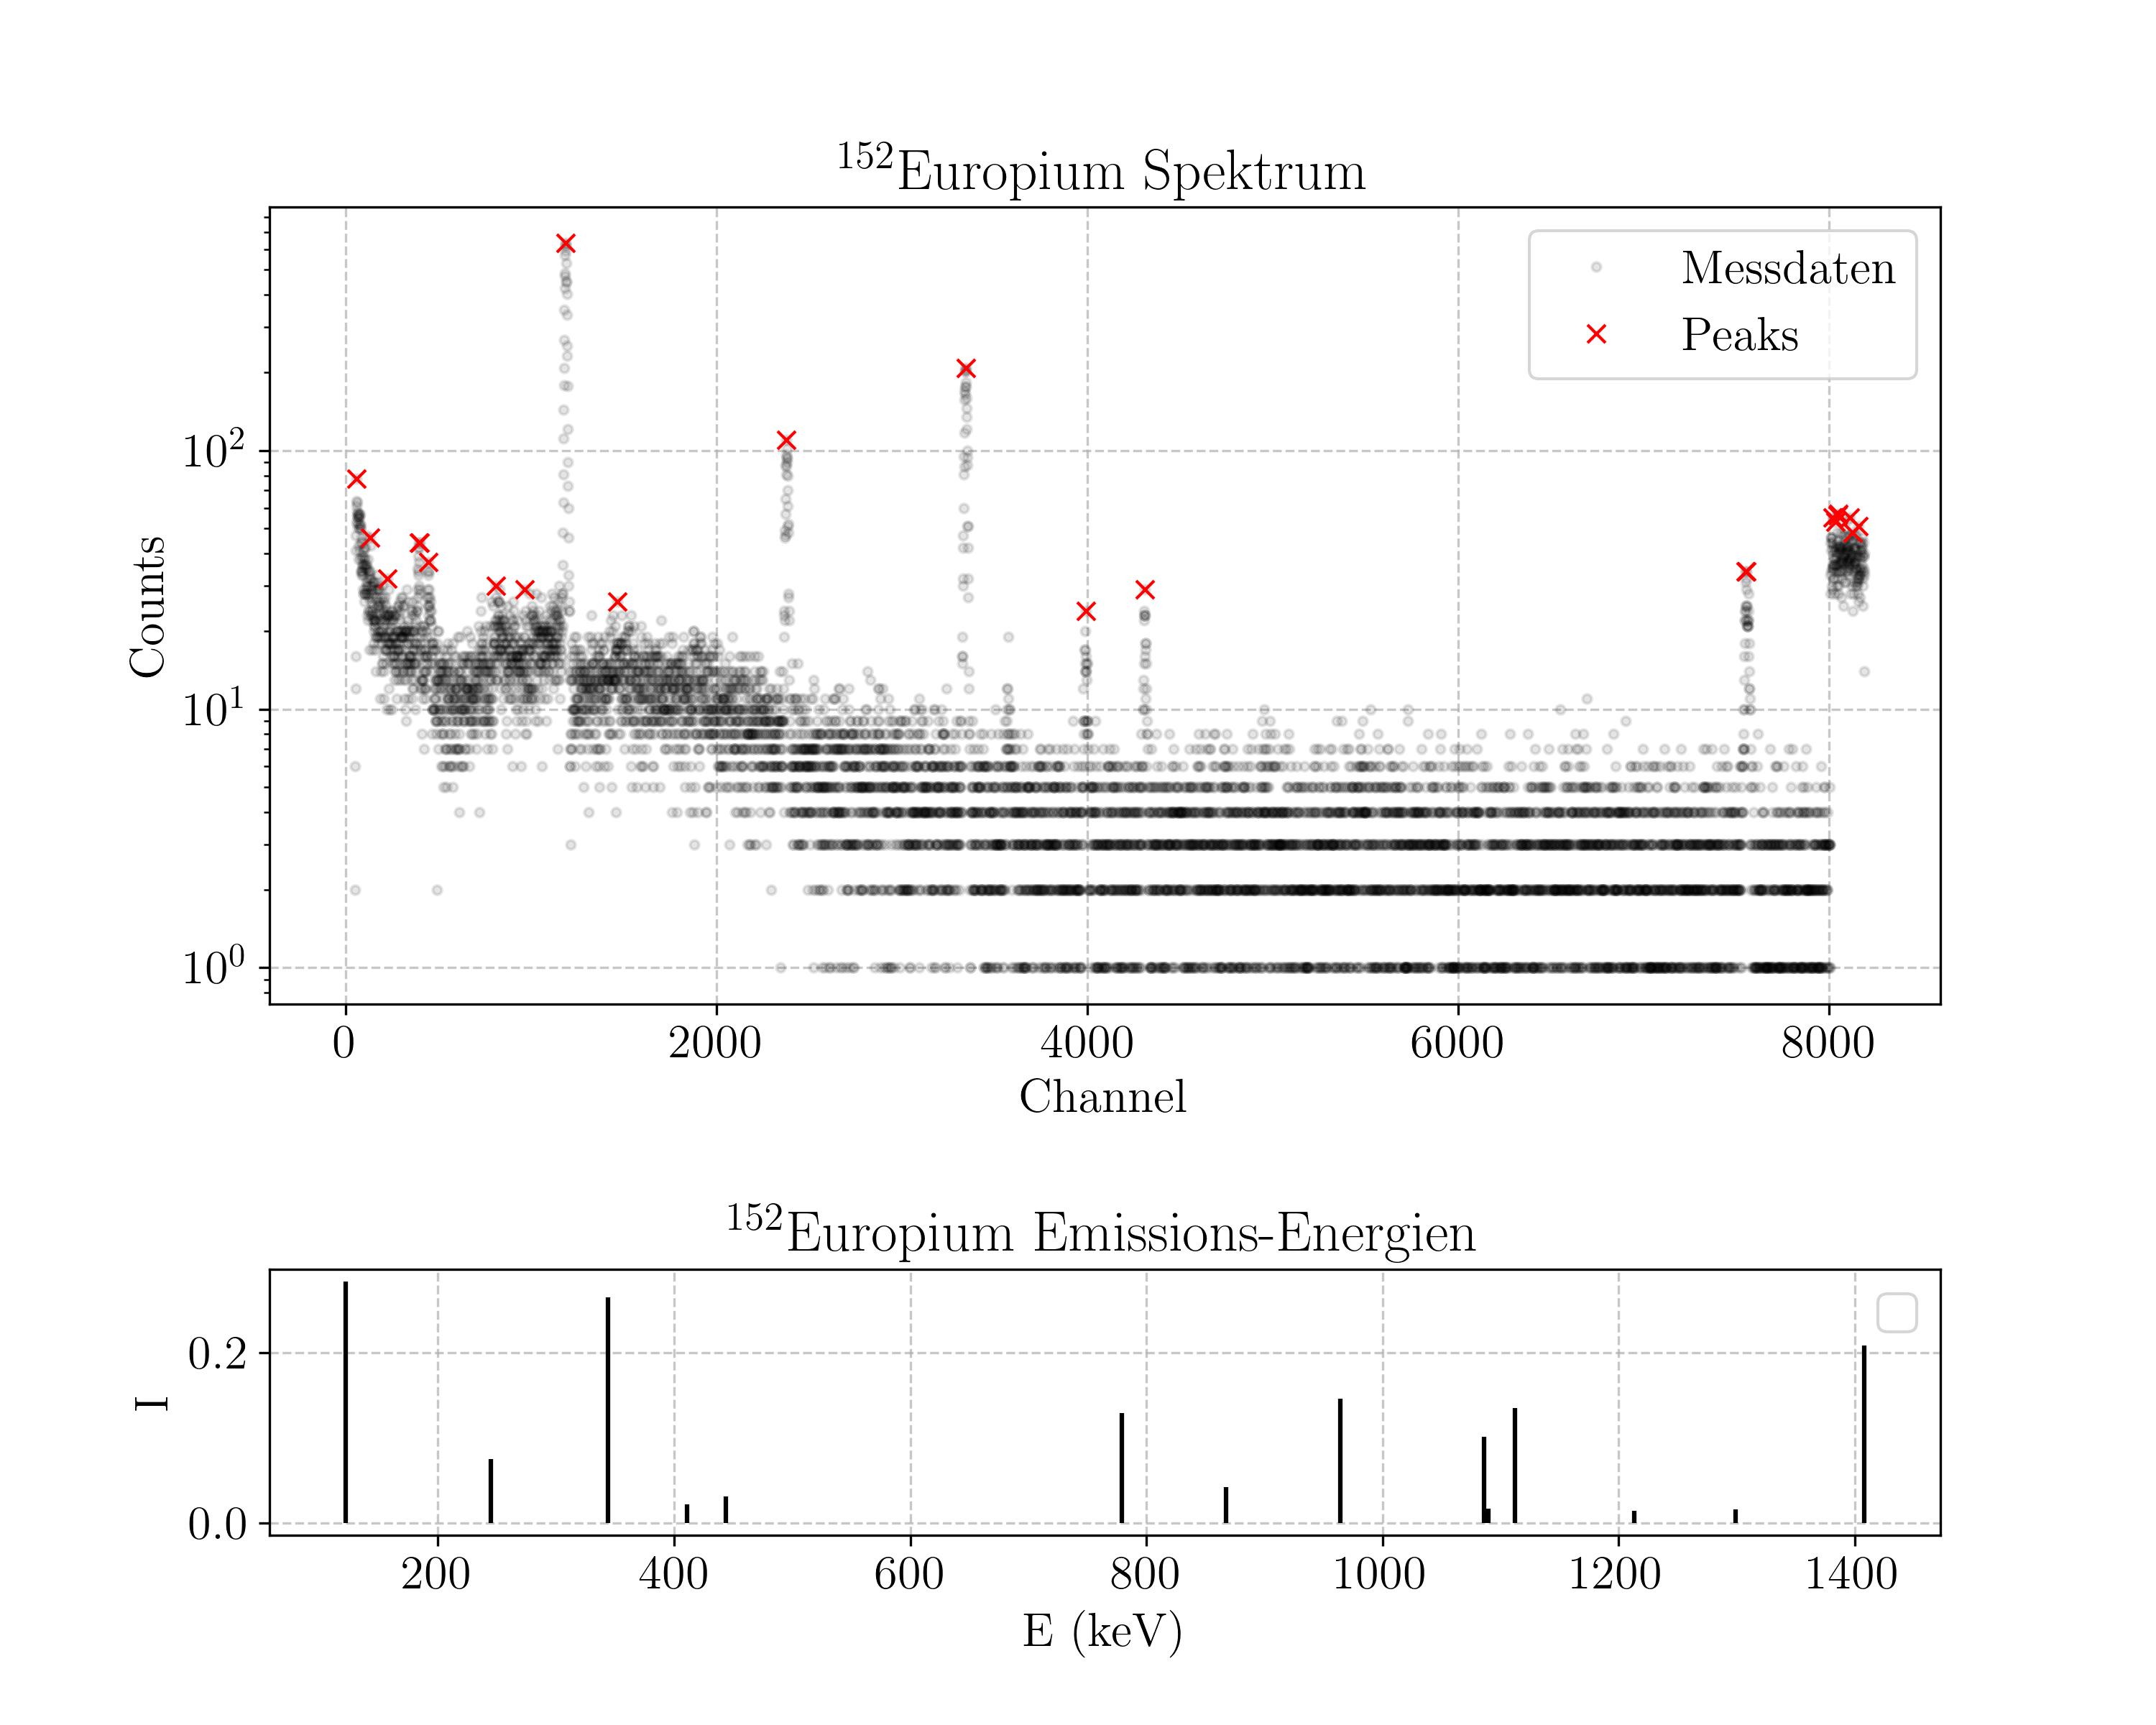
\includegraphics[scale=0.65]{Skripte/152Europium_with_emission.png}
    \caption{Messdaten des Spektrums von $\text{Eu}^{152}"$ inklusive Peaks und theoretische Emissionsenergien und Intensitäten.\cite{iaea1991}}
    \label{fig:Eu1}
  \end{figure}
Nun kann eine Auswahl von Peaks in den Daten, in \autoref{tab:peaks} aufgeführt, welche deckungsgleich zu den bekannten Theoriewerten erscheinen, zu einer Linearen Ausgleichsrechnung herangezogen werden, welche die in \autoref{fig:Eu2} dargestellte Abhängigkeit von Emissionsenergie und Messkanal innerhalb des Detektors ergibt.
\begin{figure}[H]
  \centering
  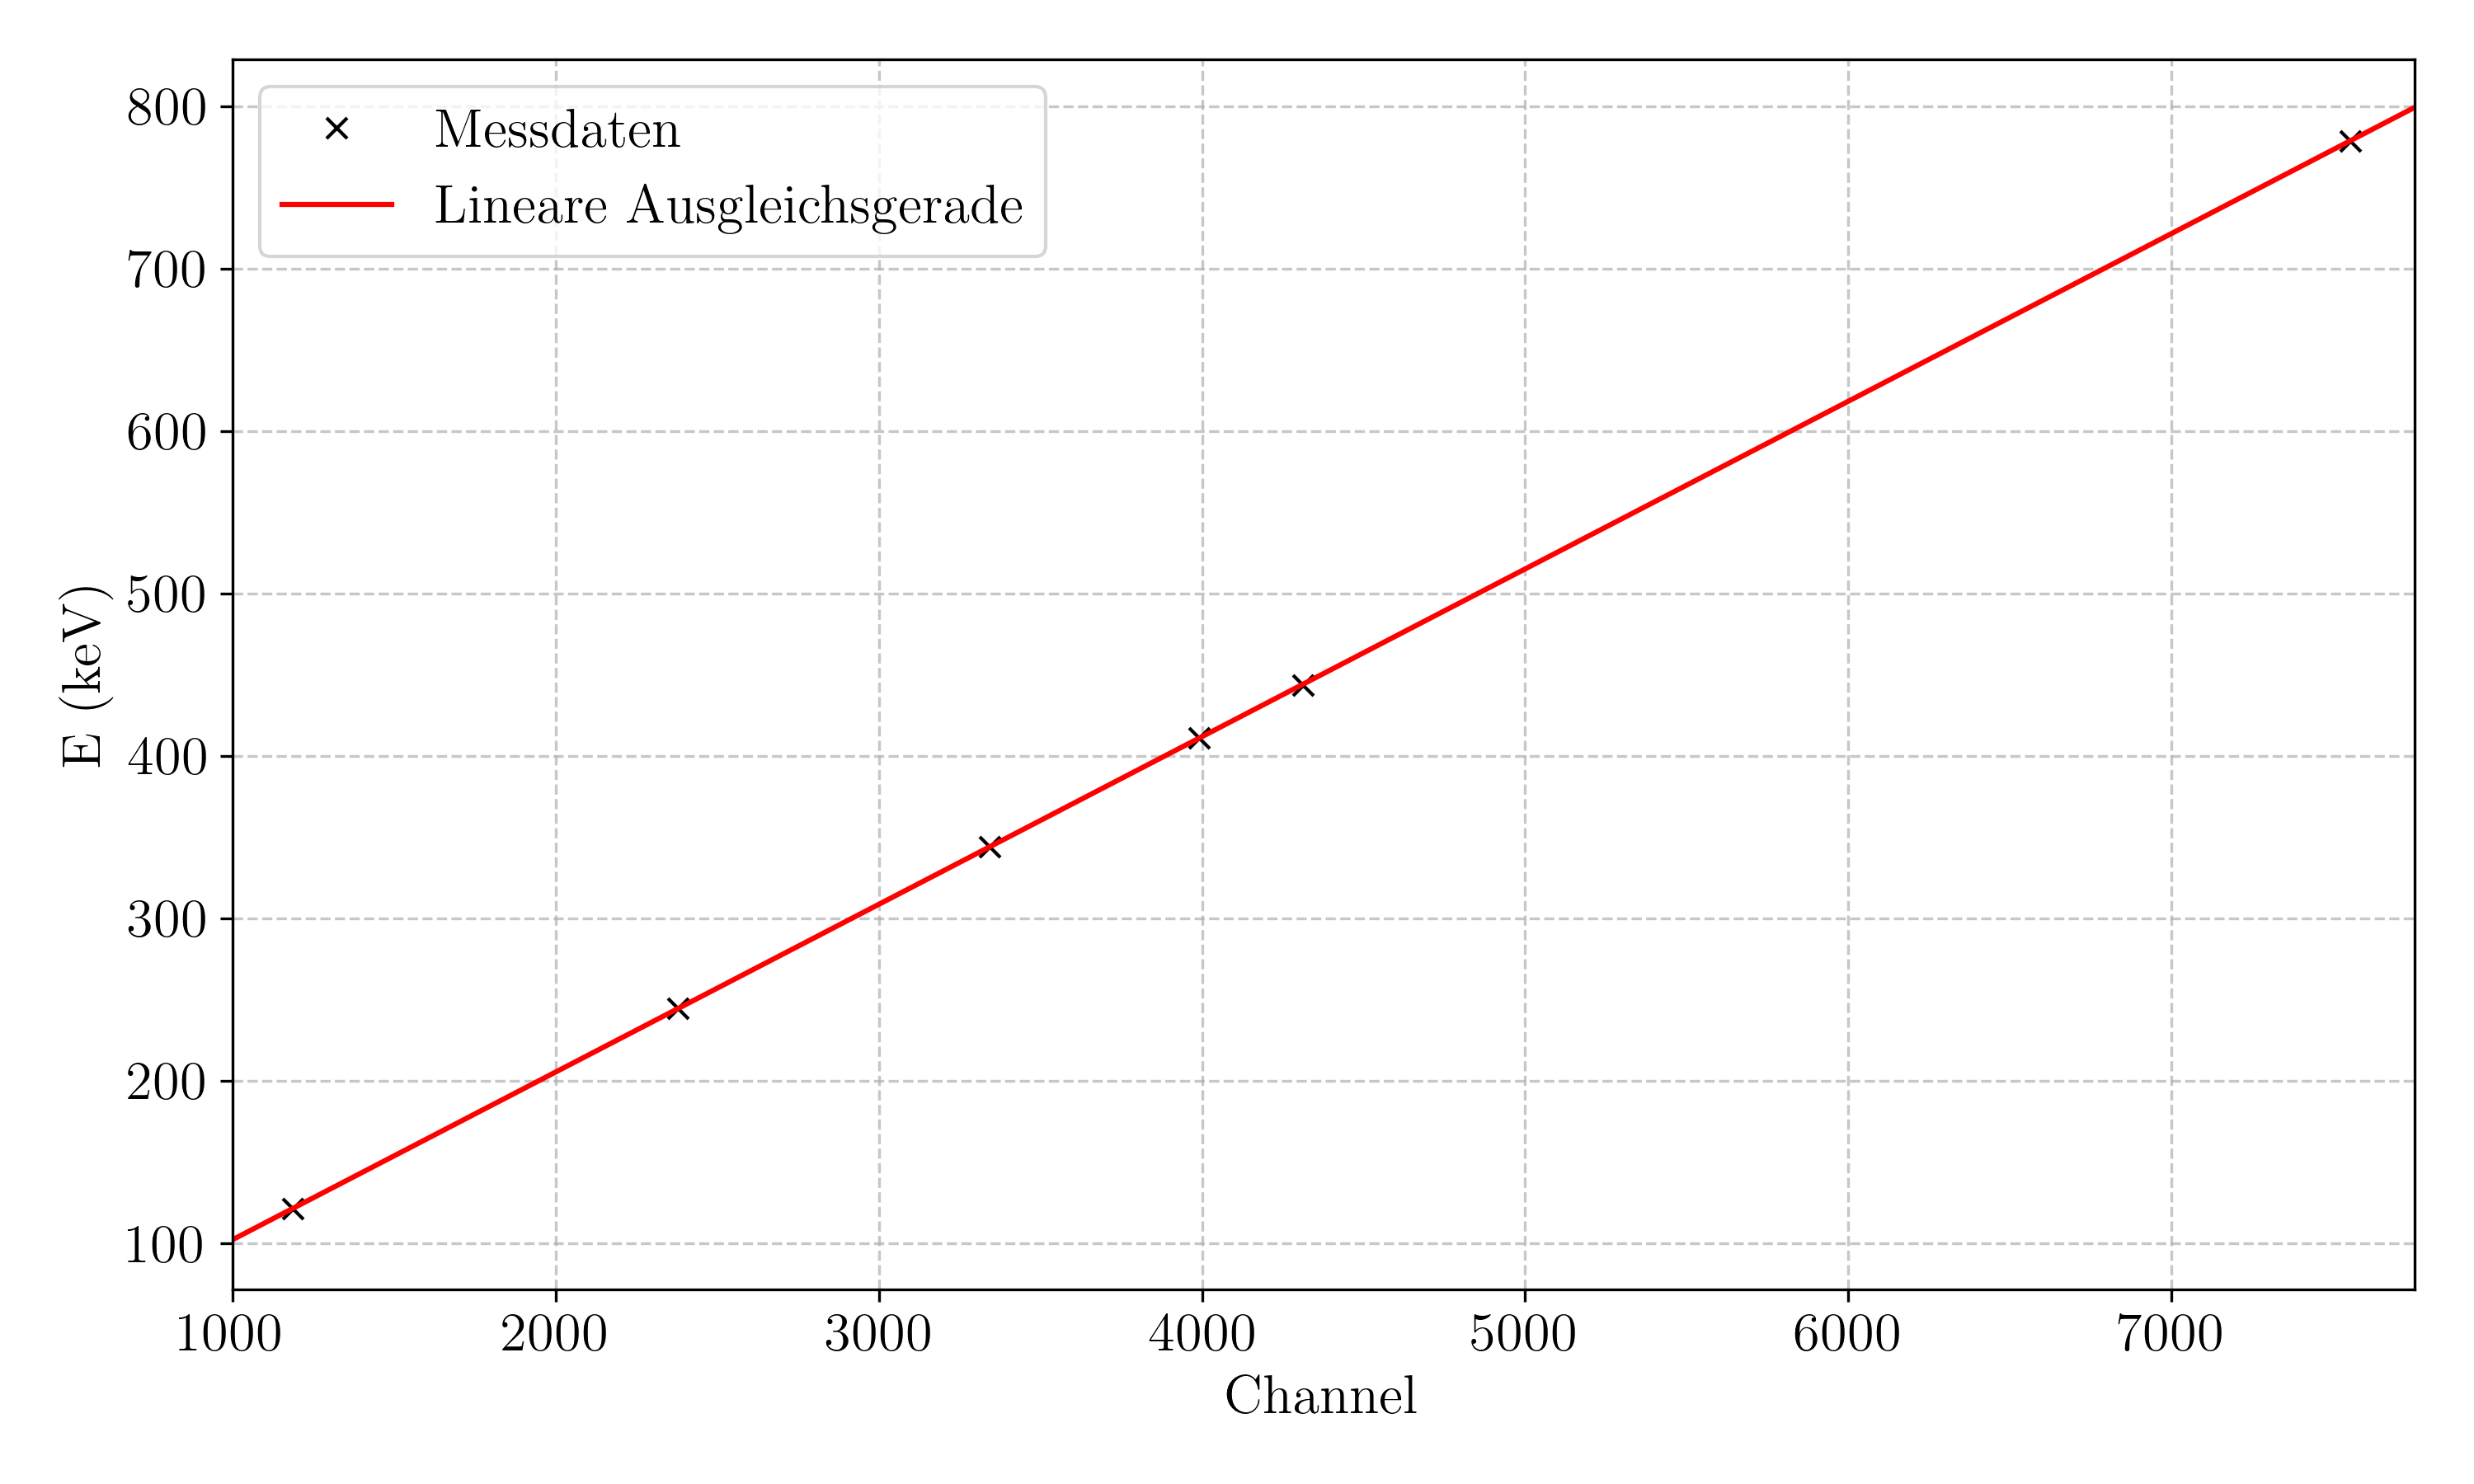
\includegraphics[scale=0.65]{Skripte/Energy_vs_Channel.png}
  \caption{Linearer Fit an Datenpaare von Messdaten und bekannten Emissionsenergien.}
  \label{fig:Eu2}
\end{figure}
\begin{table}[htbp]
  \centering
  \caption{Zugeordnete Kanalnummern zu bekannten Emissionsenergien\\von $^{152}$Eu für die Energiekalibrierung.}
  \label{tab:peaks}
  \begin{tabular}{S[table-format=3.2] c}
    \toprule
    {Theoretische Energie [\si{\kilo\electronvolt}]} & {Gemessener Kanal} \\
    \midrule
    121.78 & 1186 \\
    244.70 & 2378 \\
    344.28 & 3344 \\
    411.13 & 3992 \\
    443.97 & 4312 \\
    778.90 & 7552 \\
    \bottomrule
  \end{tabular}
\end{table}
Als Parameter für die Funktion
\begin{align*}
  E(K)=m\cdot K + b\text{,}
\end{align*}
wobei $K$ die Kanalnummer angibt, ergeben sich
\begin{align}
  m&=\SI{0.1032}{\kilo\eV}\\
  b&=\SI{-0.8336}{\kilo\eV}\text{.}
\end{align}
Wenn nun an die Ausgewählten Peaks Gaussfunktionen angepasst werden, wie beispielhaft in \autoref{fig:Eu4} dargestellt, und der Inhalt $N$ der Verteilungen gemessen wird, kann die Vollenergienachweiswahrscheinlichkeit mittels der Gleichung
\begin{align}
  Q=\frac{N}{AWt}\frac{4\pi}{\Omega}\label{eqn:Q}
\end{align}
bestimmt werden.
\begin{figure}[H]
  \centering
  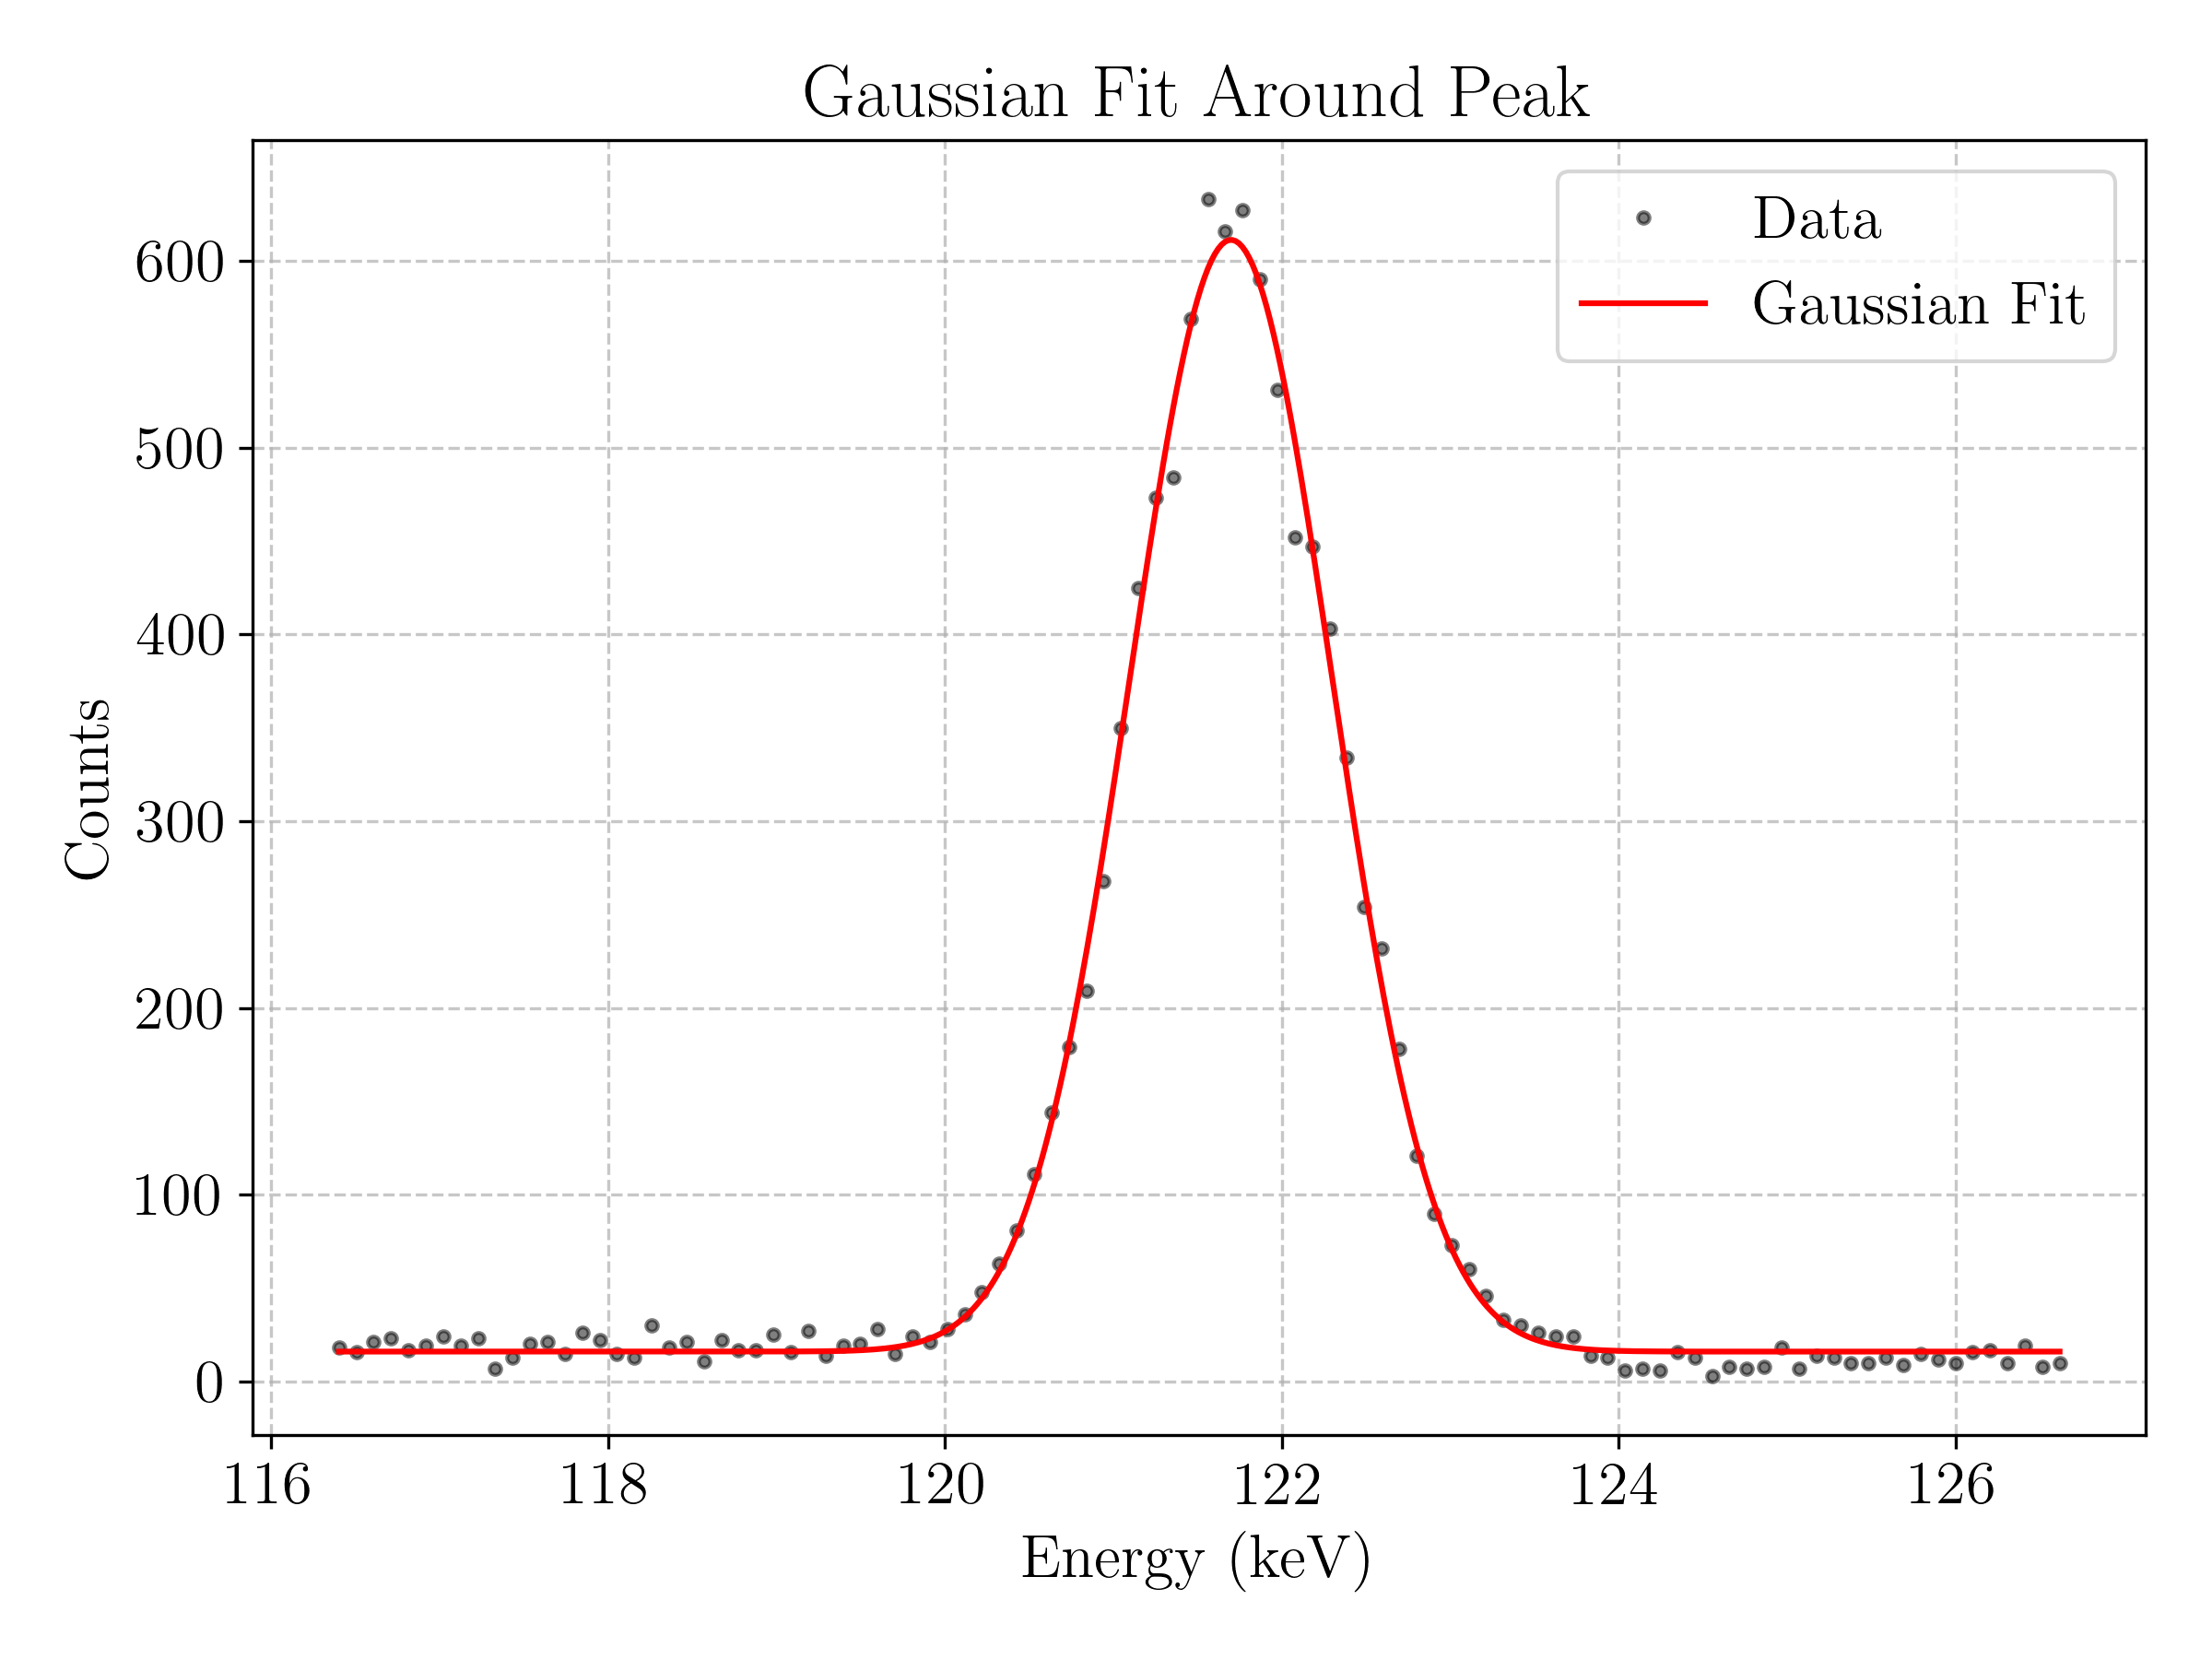
\includegraphics[scale=0.65]{Skripte/fep.png}
  \caption{Beispielhafte Gaussfunktion am \SI{122}{\kilo\eV}-Peak.}
  \label{fig:Eu4}
\end{figure}
Hierbei gibt $A$ die Aktivität der Probe am Tag der Messung, $W$ die Wahrscheinlichkeit der Emission, $t$ die Zeitspanne der Messung und $\Omega$ den Raumwinkelanteil des Detektors bezüglich der Probe an.
Die Aktivität lässt sich entsprechend
\begin{align}
  A(t)=A_0\exp{\left(-\frac{\ln{2}}{T_{1/2}} \cdot t\right)}\text{,}
\end{align}
wobei
\begin{align*}
  A_0 = \SI{4130(60)}{\becquerel}
\end{align*}
die Aktivität der Probe am 01.01.2000 ist\cite{anleitung} und 
\begin{align*}
  T_{1/2}=\SI{4934}{\day}
\end{align*}
die Halbwertszeit von Eu-152 beschreibt\cite{Kondev2021}.
Somit ergibt sich für den Tag des Versuchs eine Aktivität von
\begin{align*}
  A=\SI{1176(17)}{\becquerel}\text{.}
\end{align*}
Der Raumwinkelanteil lässt sich gemäß der Geometrie in \autoref{fig:detector} zu
\begin{align*}
  \Omega=0,0167\pm0.0004
\end{align*}
bestimmen.
An die mit \autoref{eqn:Q} bestimmten Vollenergienachweiswahrscheinlichkeiten kann nun eine Exponentialfunktion des Schemas
\begin{align*}
  Q_\text{fit}(E)=a\cdot b^E+c
\end{align*}
mittels SciPy angepasst werden.
Es ergeben sich die Parameter
\begin{align}
  a &= 0.0945\pm0.0040\\
   b &= 0.9952\pm0.0.0004\\
    c &= 0.0078\pm0.0017
\end{align}
und die Funktion ist mit den Werten in \autoref{fig:Q} dargestellt.
\begin{figure}[H]
  \centering
  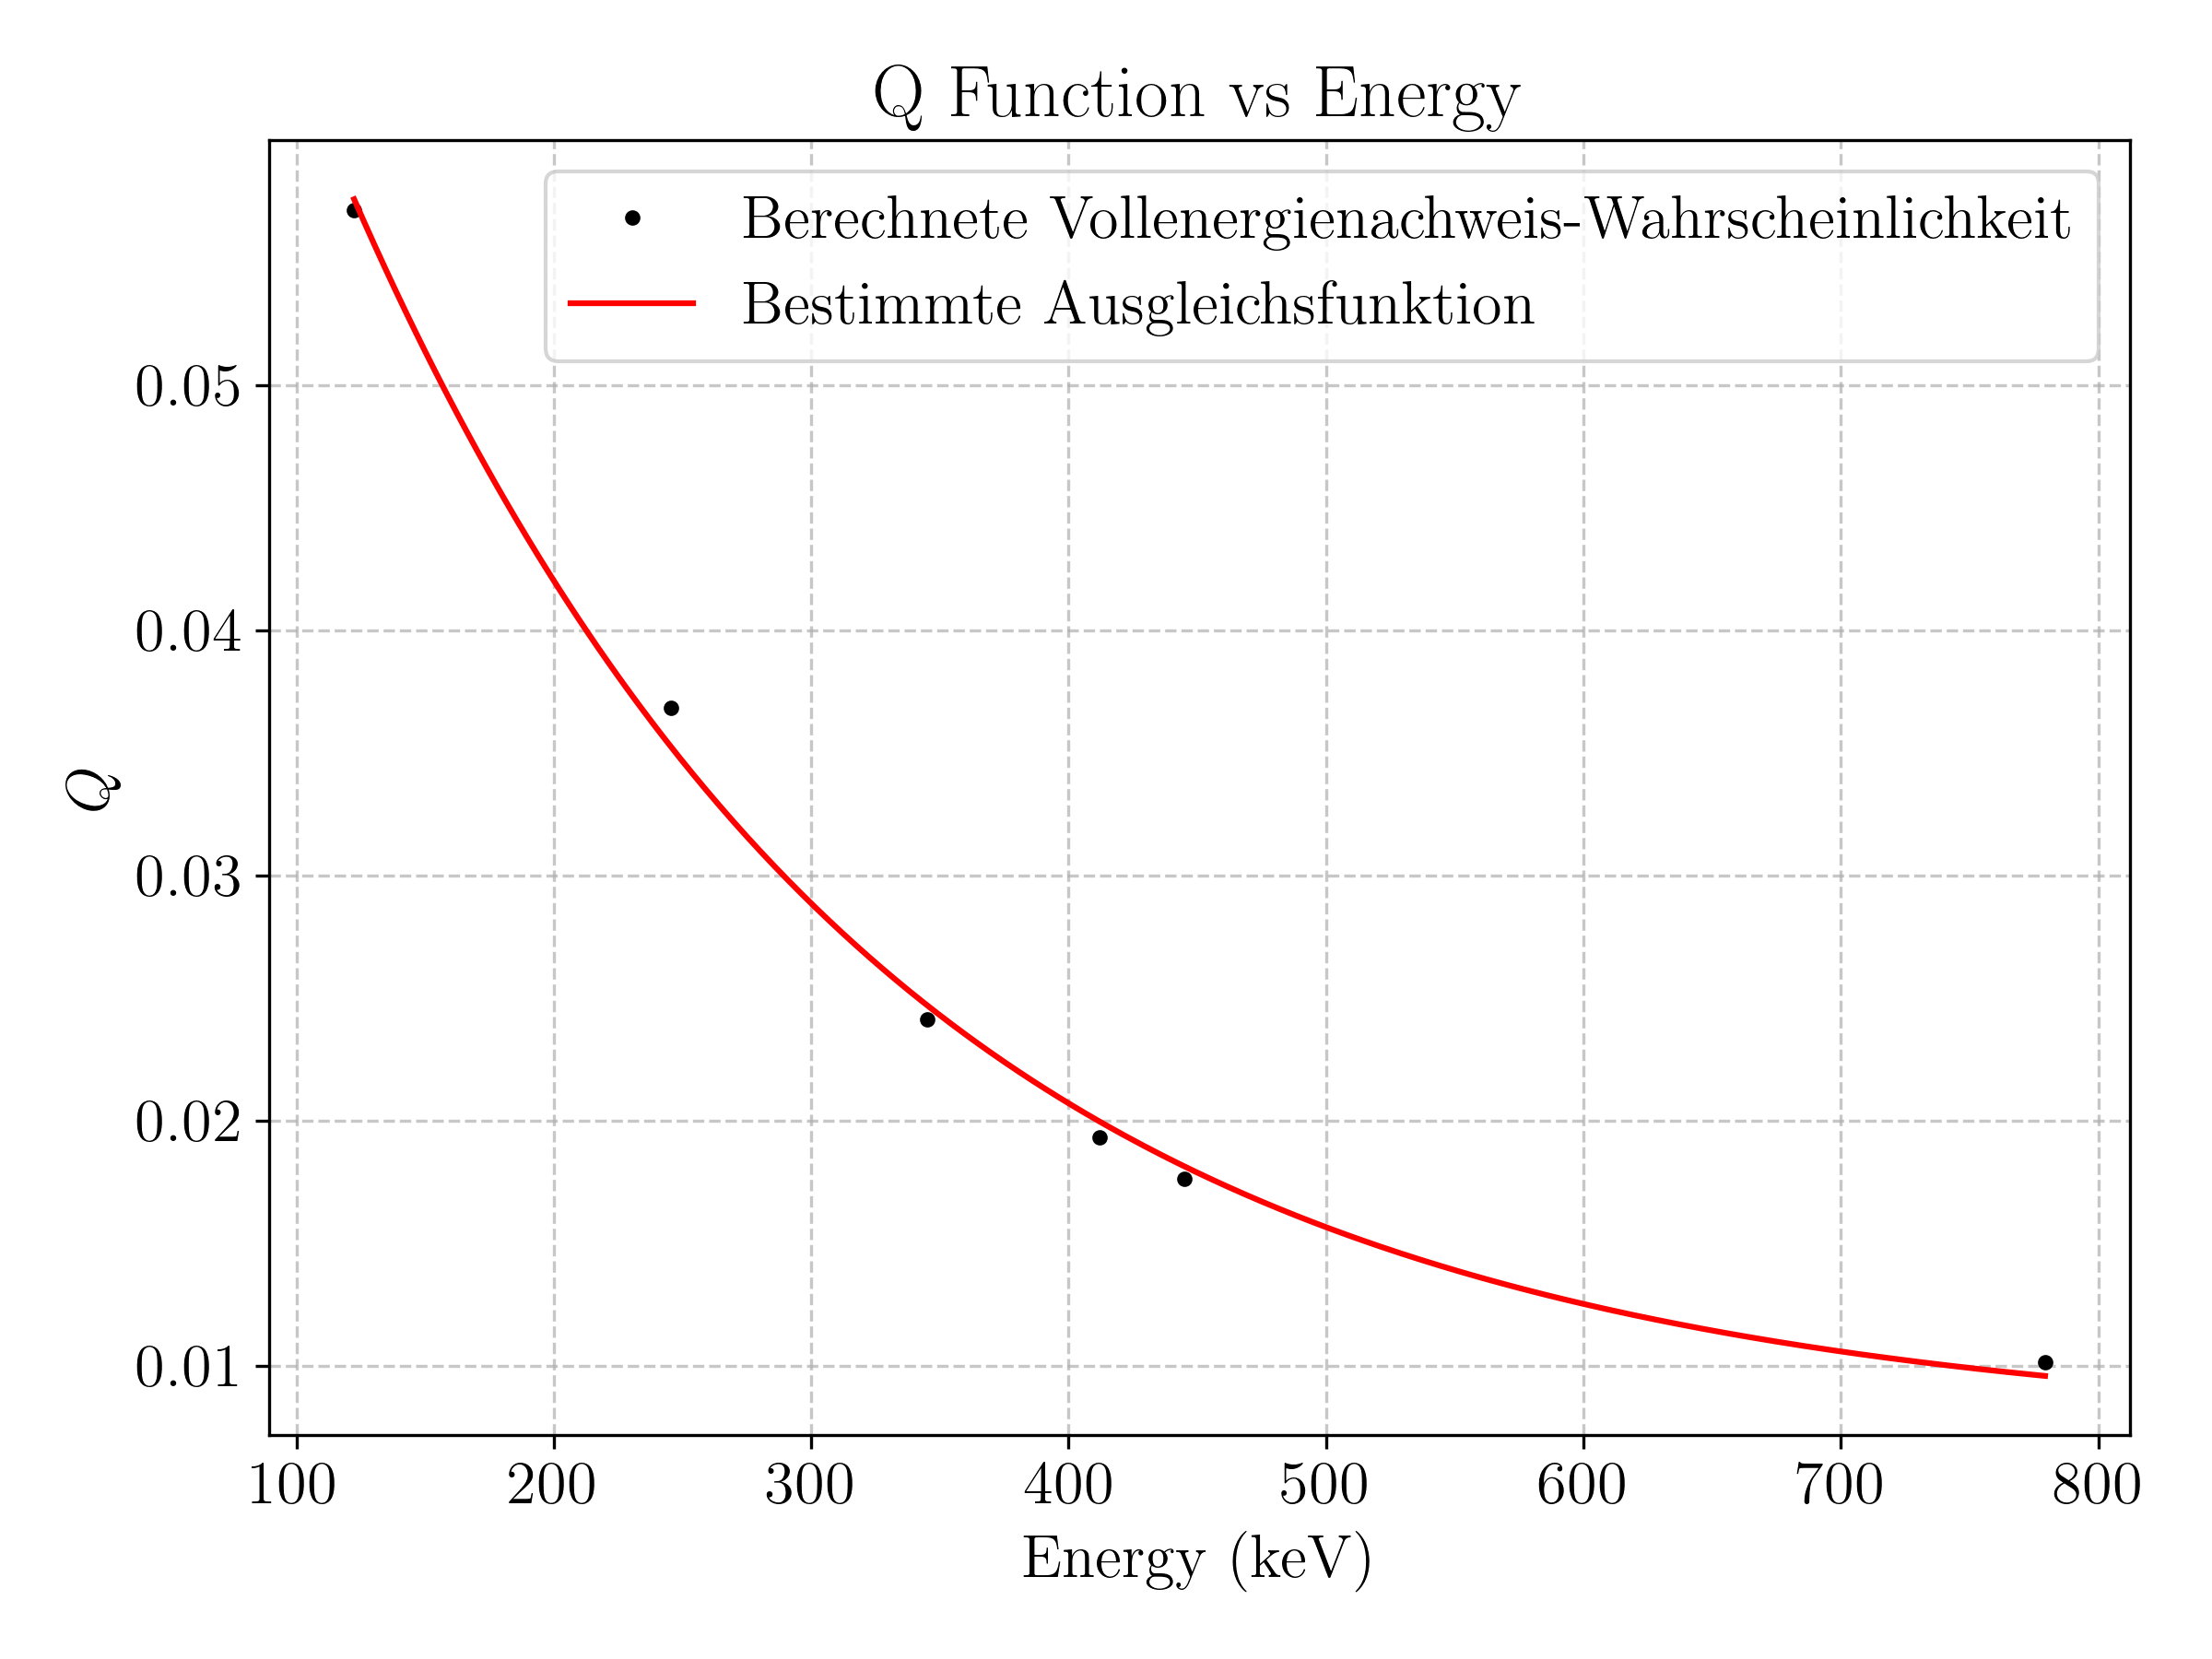
\includegraphics[scale=0.65]{Skripte/Qfunc.png}
  \caption{Berechnete Vollenergienachweiswahrscheinlichkeiten mit angepasster e-Funktion.}
  \label{fig:Q}
\end{figure}
Mittels der nun bestimmten Funtion können die Messdaten nachträglich korrigiert werden, indem die Anzahl der Counts durch den zugehörigen Wert der Funktion geteilt werden.
In \autoref{fig:Eu3} sind die Ausgewählten Peaks, nun mit den Energien anstelle der Kanalnummern und die Korrektur durch die Vollenergienachweiswahrscheinlichkeit zu sehen. 
\begin{figure}[H]
  \centering
  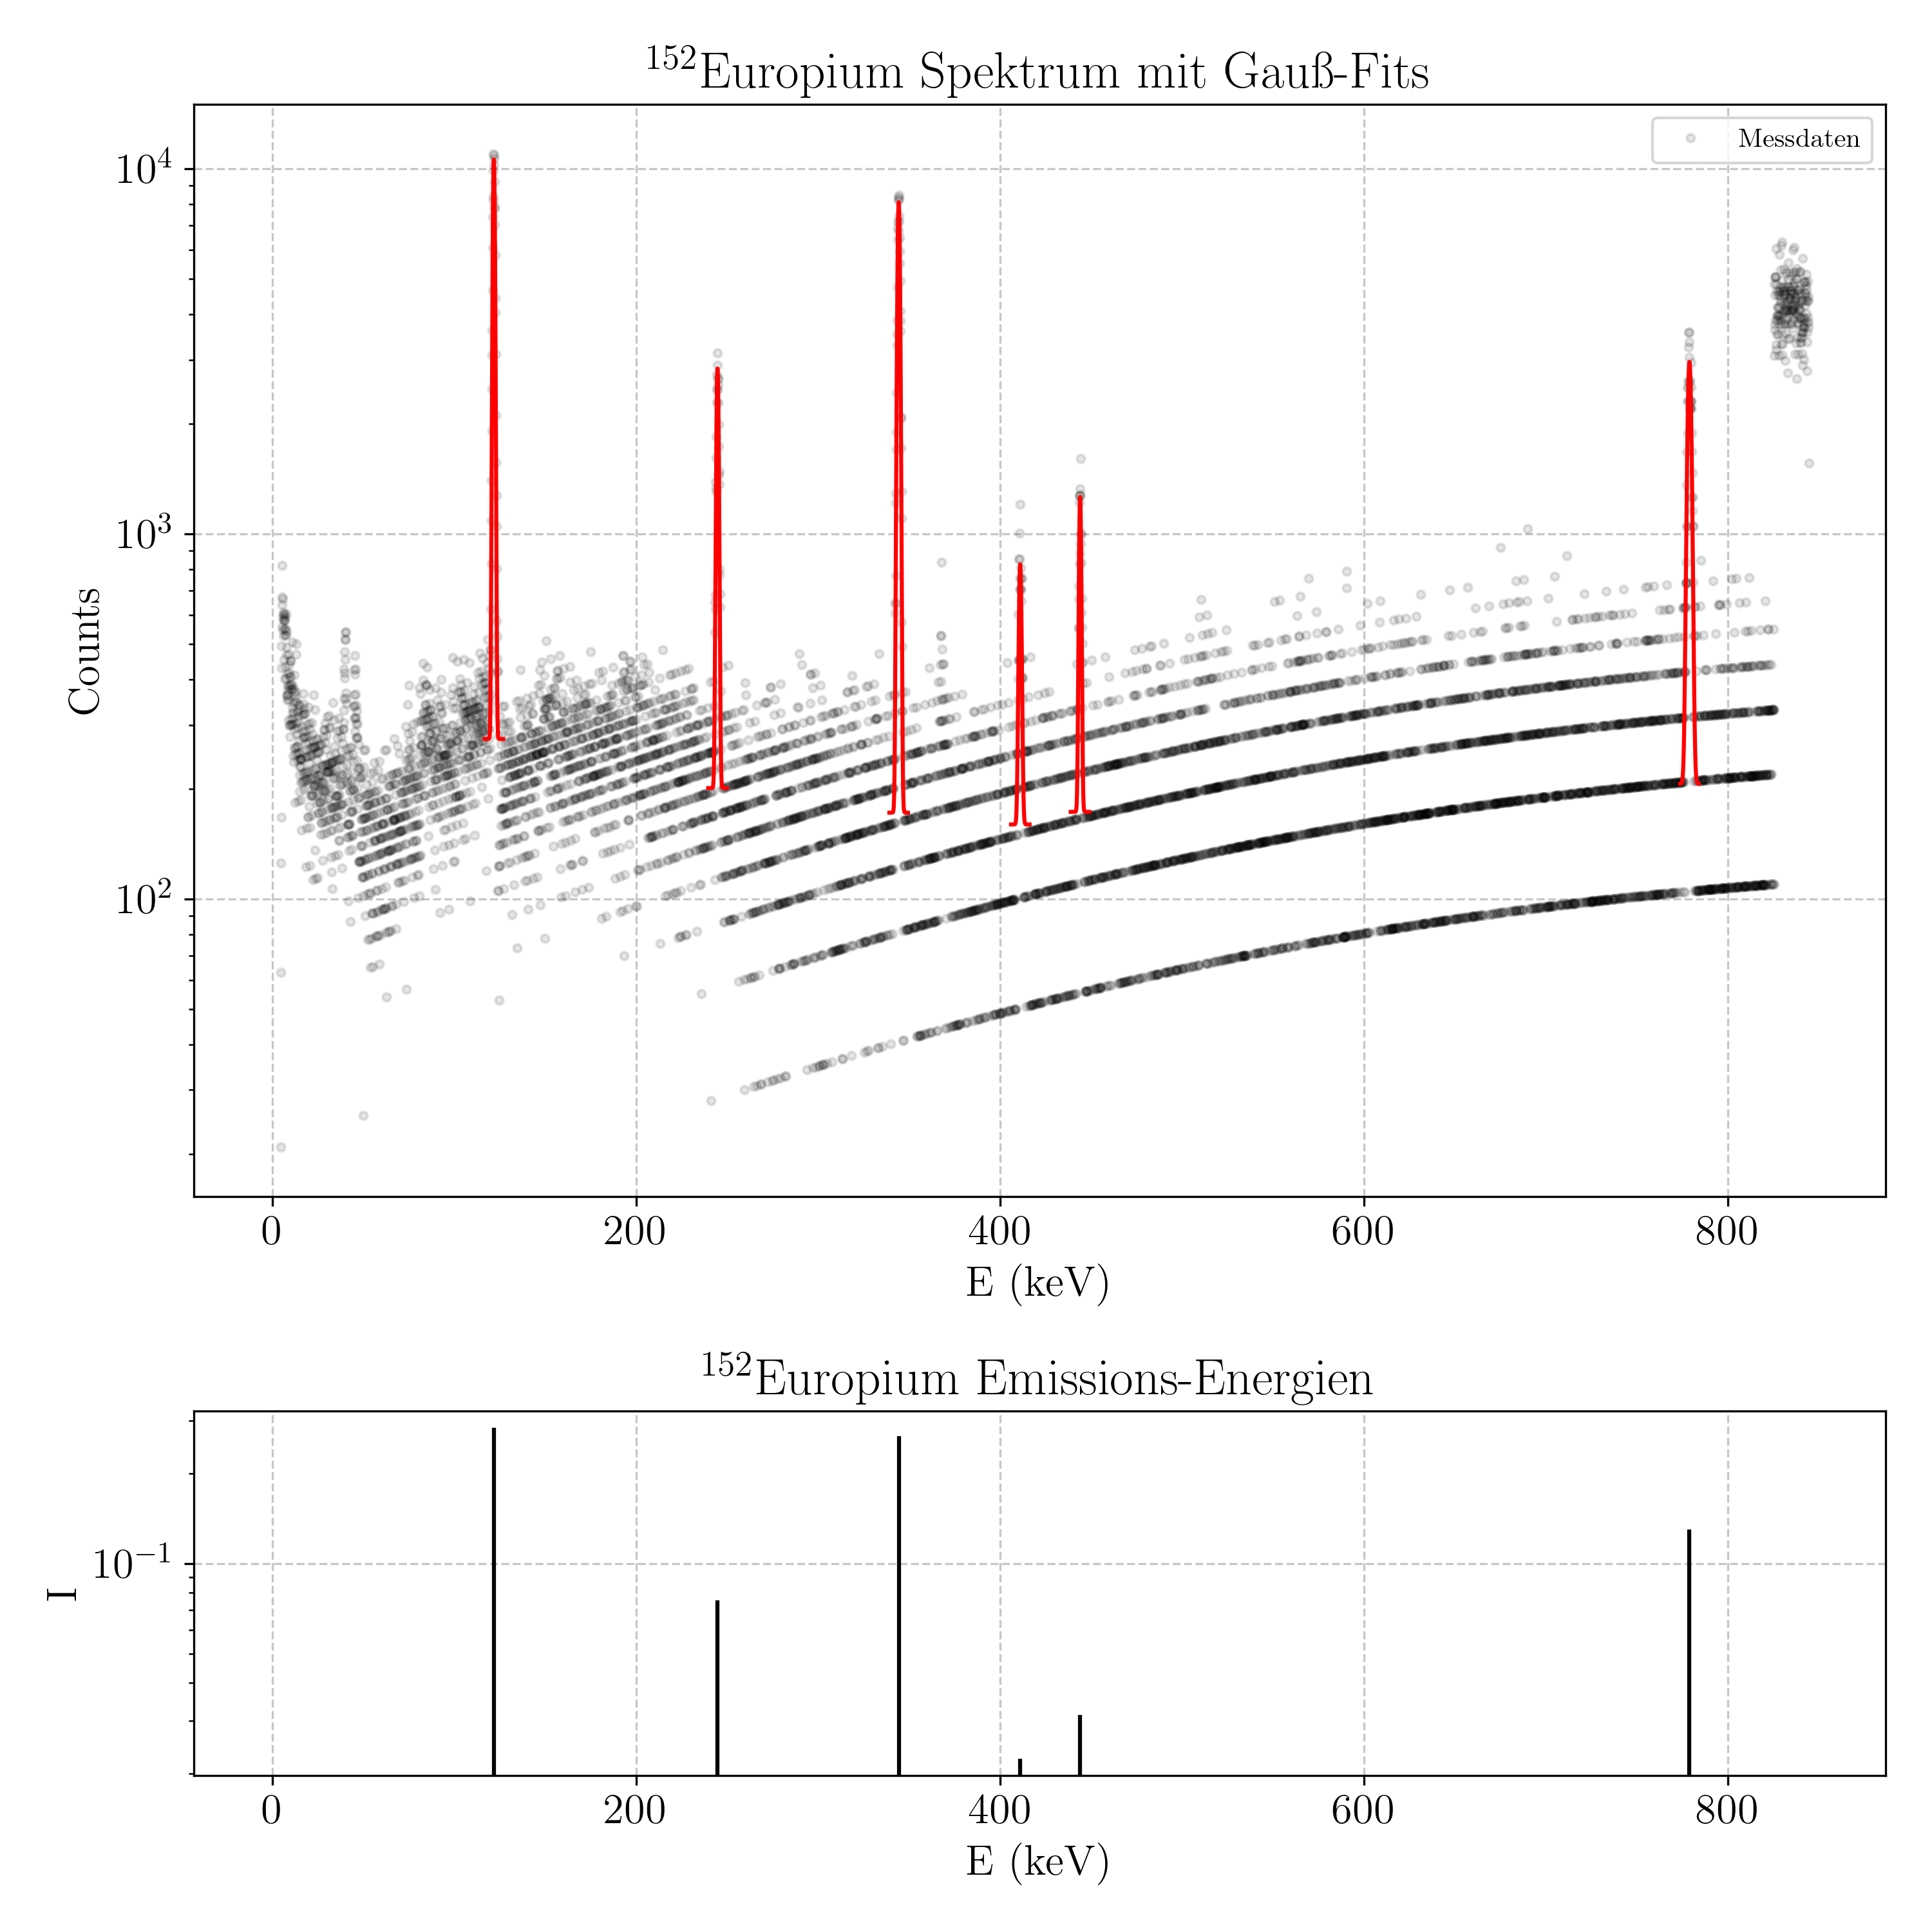
\includegraphics[scale=0.65]{Skripte/152Europium_with_Gaussians_and_Energies.png}
  \caption{Messspektrum in Abhängigkeit der Energie mit Gaussfunktionen angepasst an die relevanten Peaks.}
  \label{fig:Eu3}
\end{figure}
\newpage
\subsection{Untersuchung eines monochromatischen Gamma-Spektrums}
Für diesen Teil des Versuchs wurde eine $\text{Cs}^{137}$-Quelle vermessen, die Messdaten sind in \autoref{fig:Cs1} inklusive Full-Energy-Peak dargestellt.
\begin{figure}[H]
  \centering
  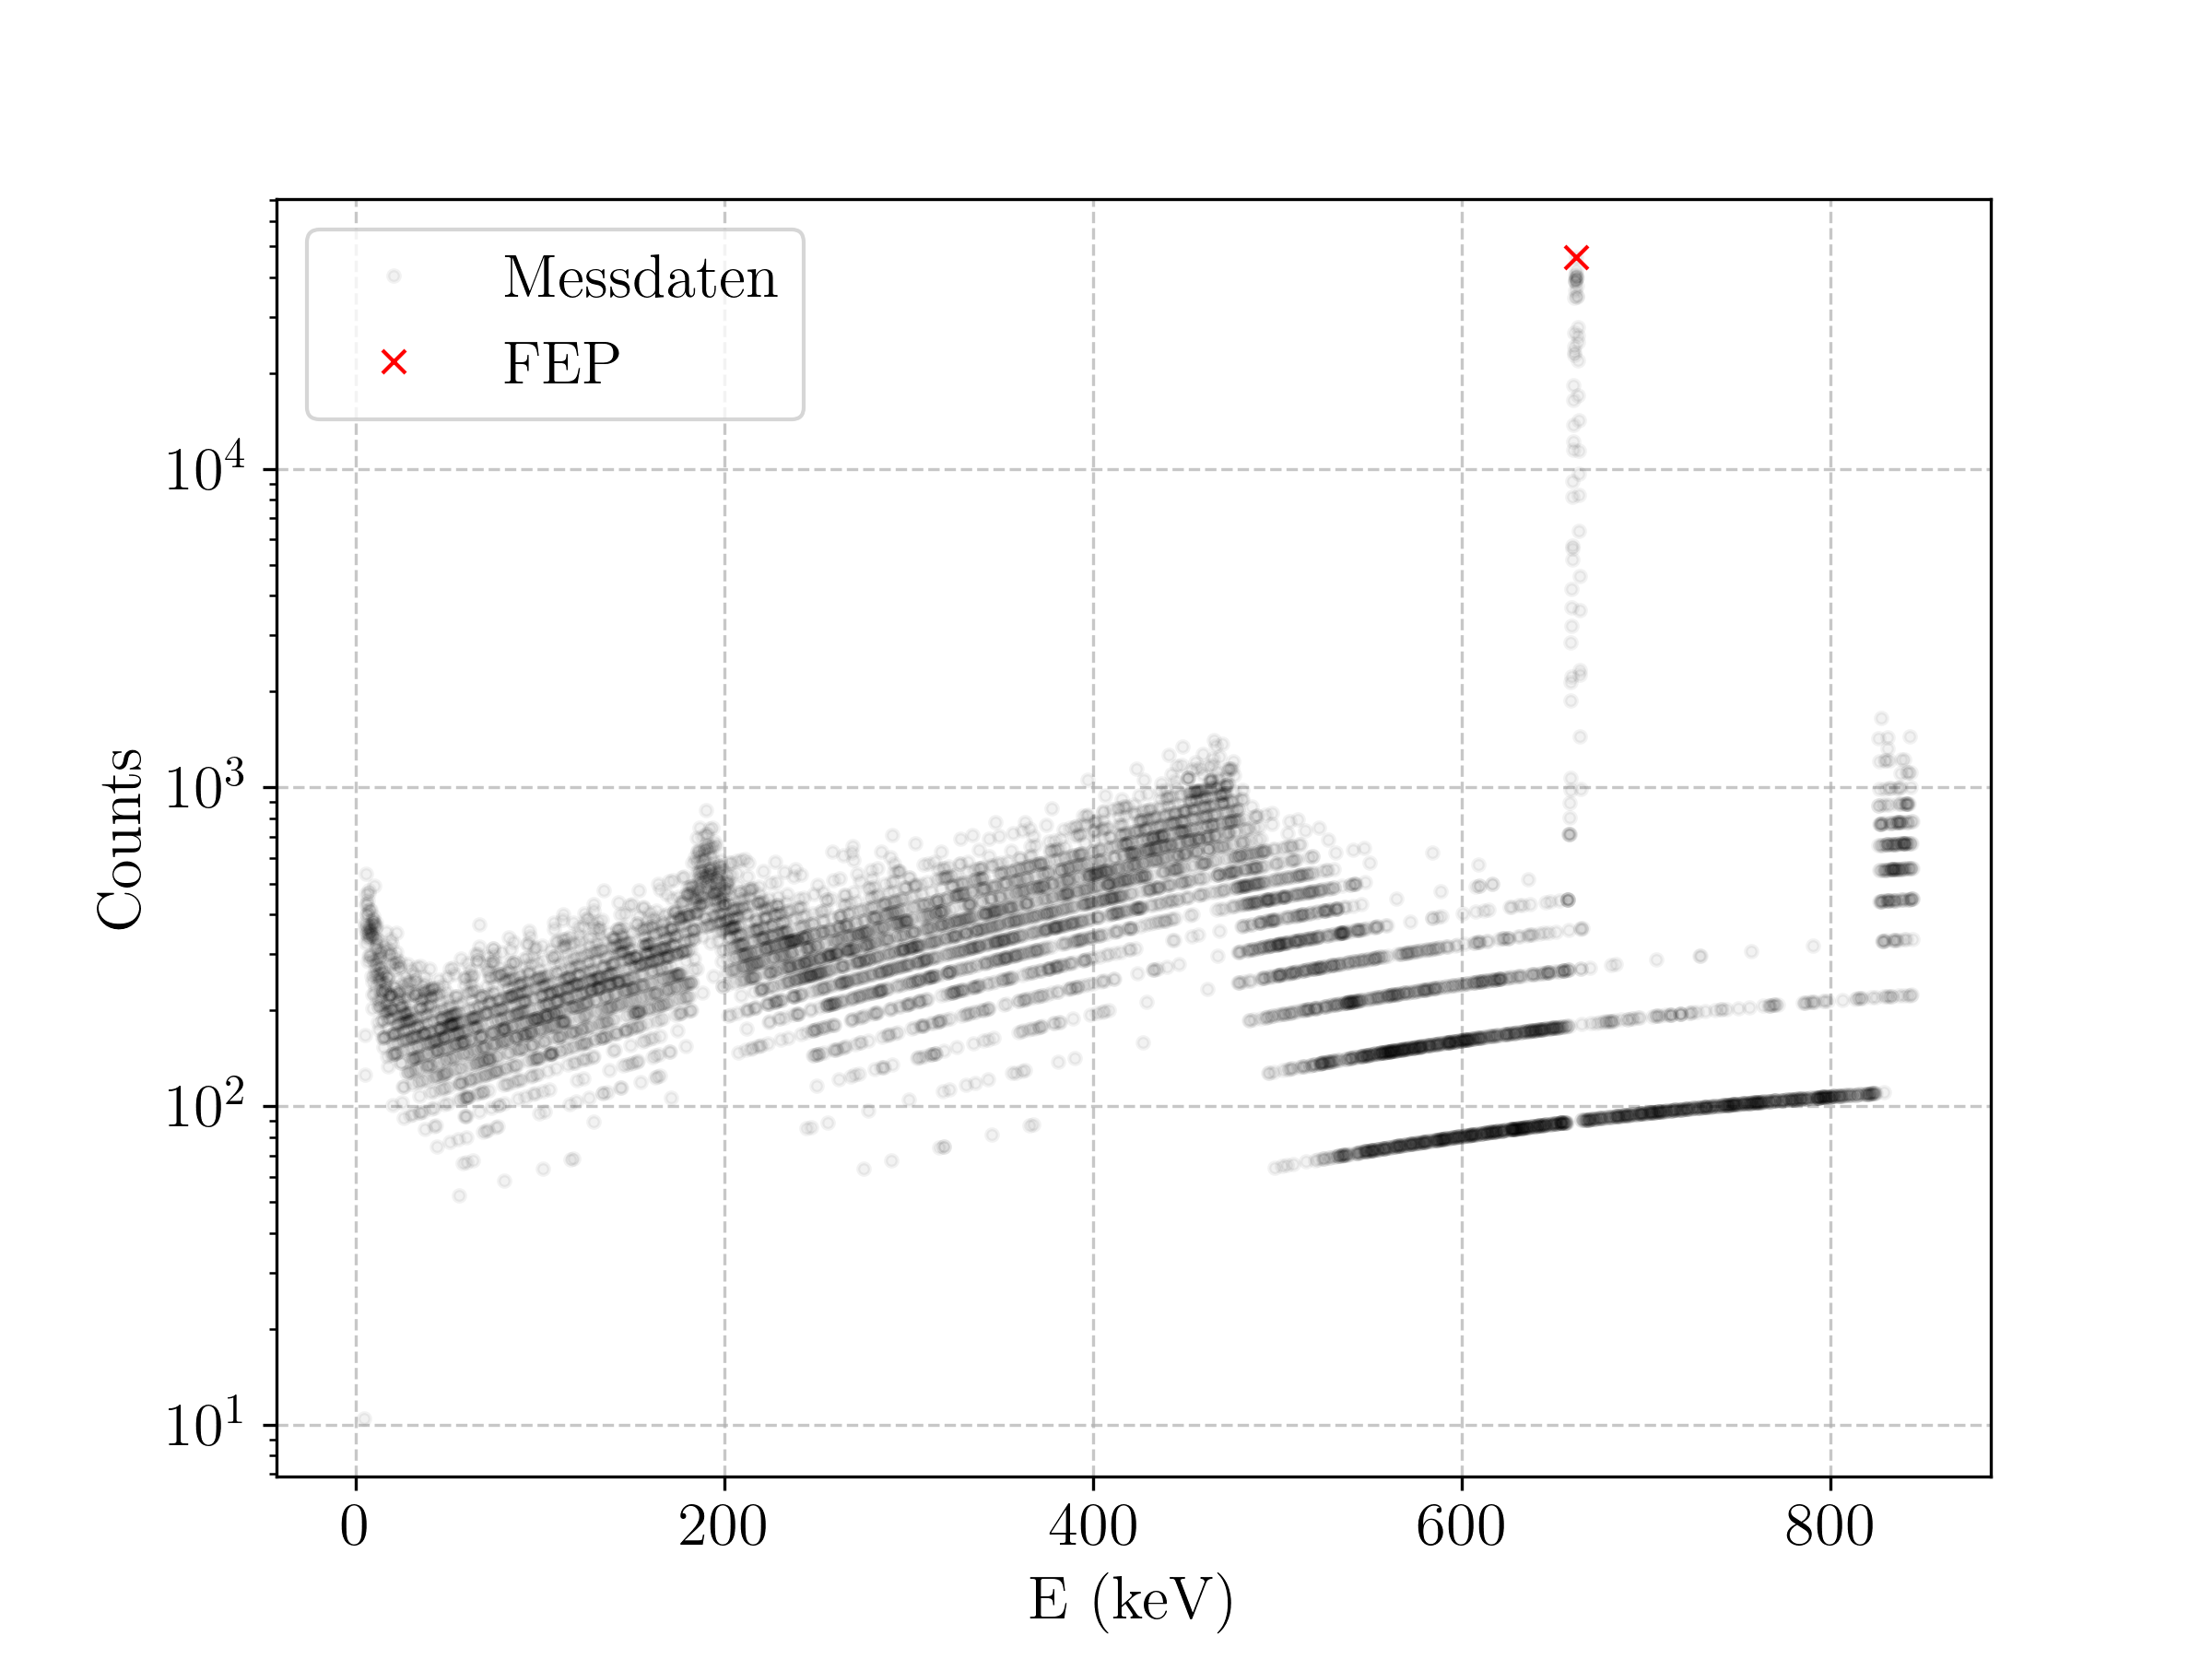
\includegraphics[scale=0.65]{Skripte/137Caesium_original.png}
  \caption{Messspektrum der $\text{Cs}^{137}$-Quelle}
  \label{fig:Cs1}
\end{figure}
Der Full-Energy-Peak und eine angepasste Gaußfunktion im konkreten sind in \autoref{fig:Cs2} zu sehen, des Weiteren sind Halbwertsbreite (FWHM) und Zehntelwertsbreite (FWTM) eingezeichnet.
\begin{figure}[H]
  \centering
  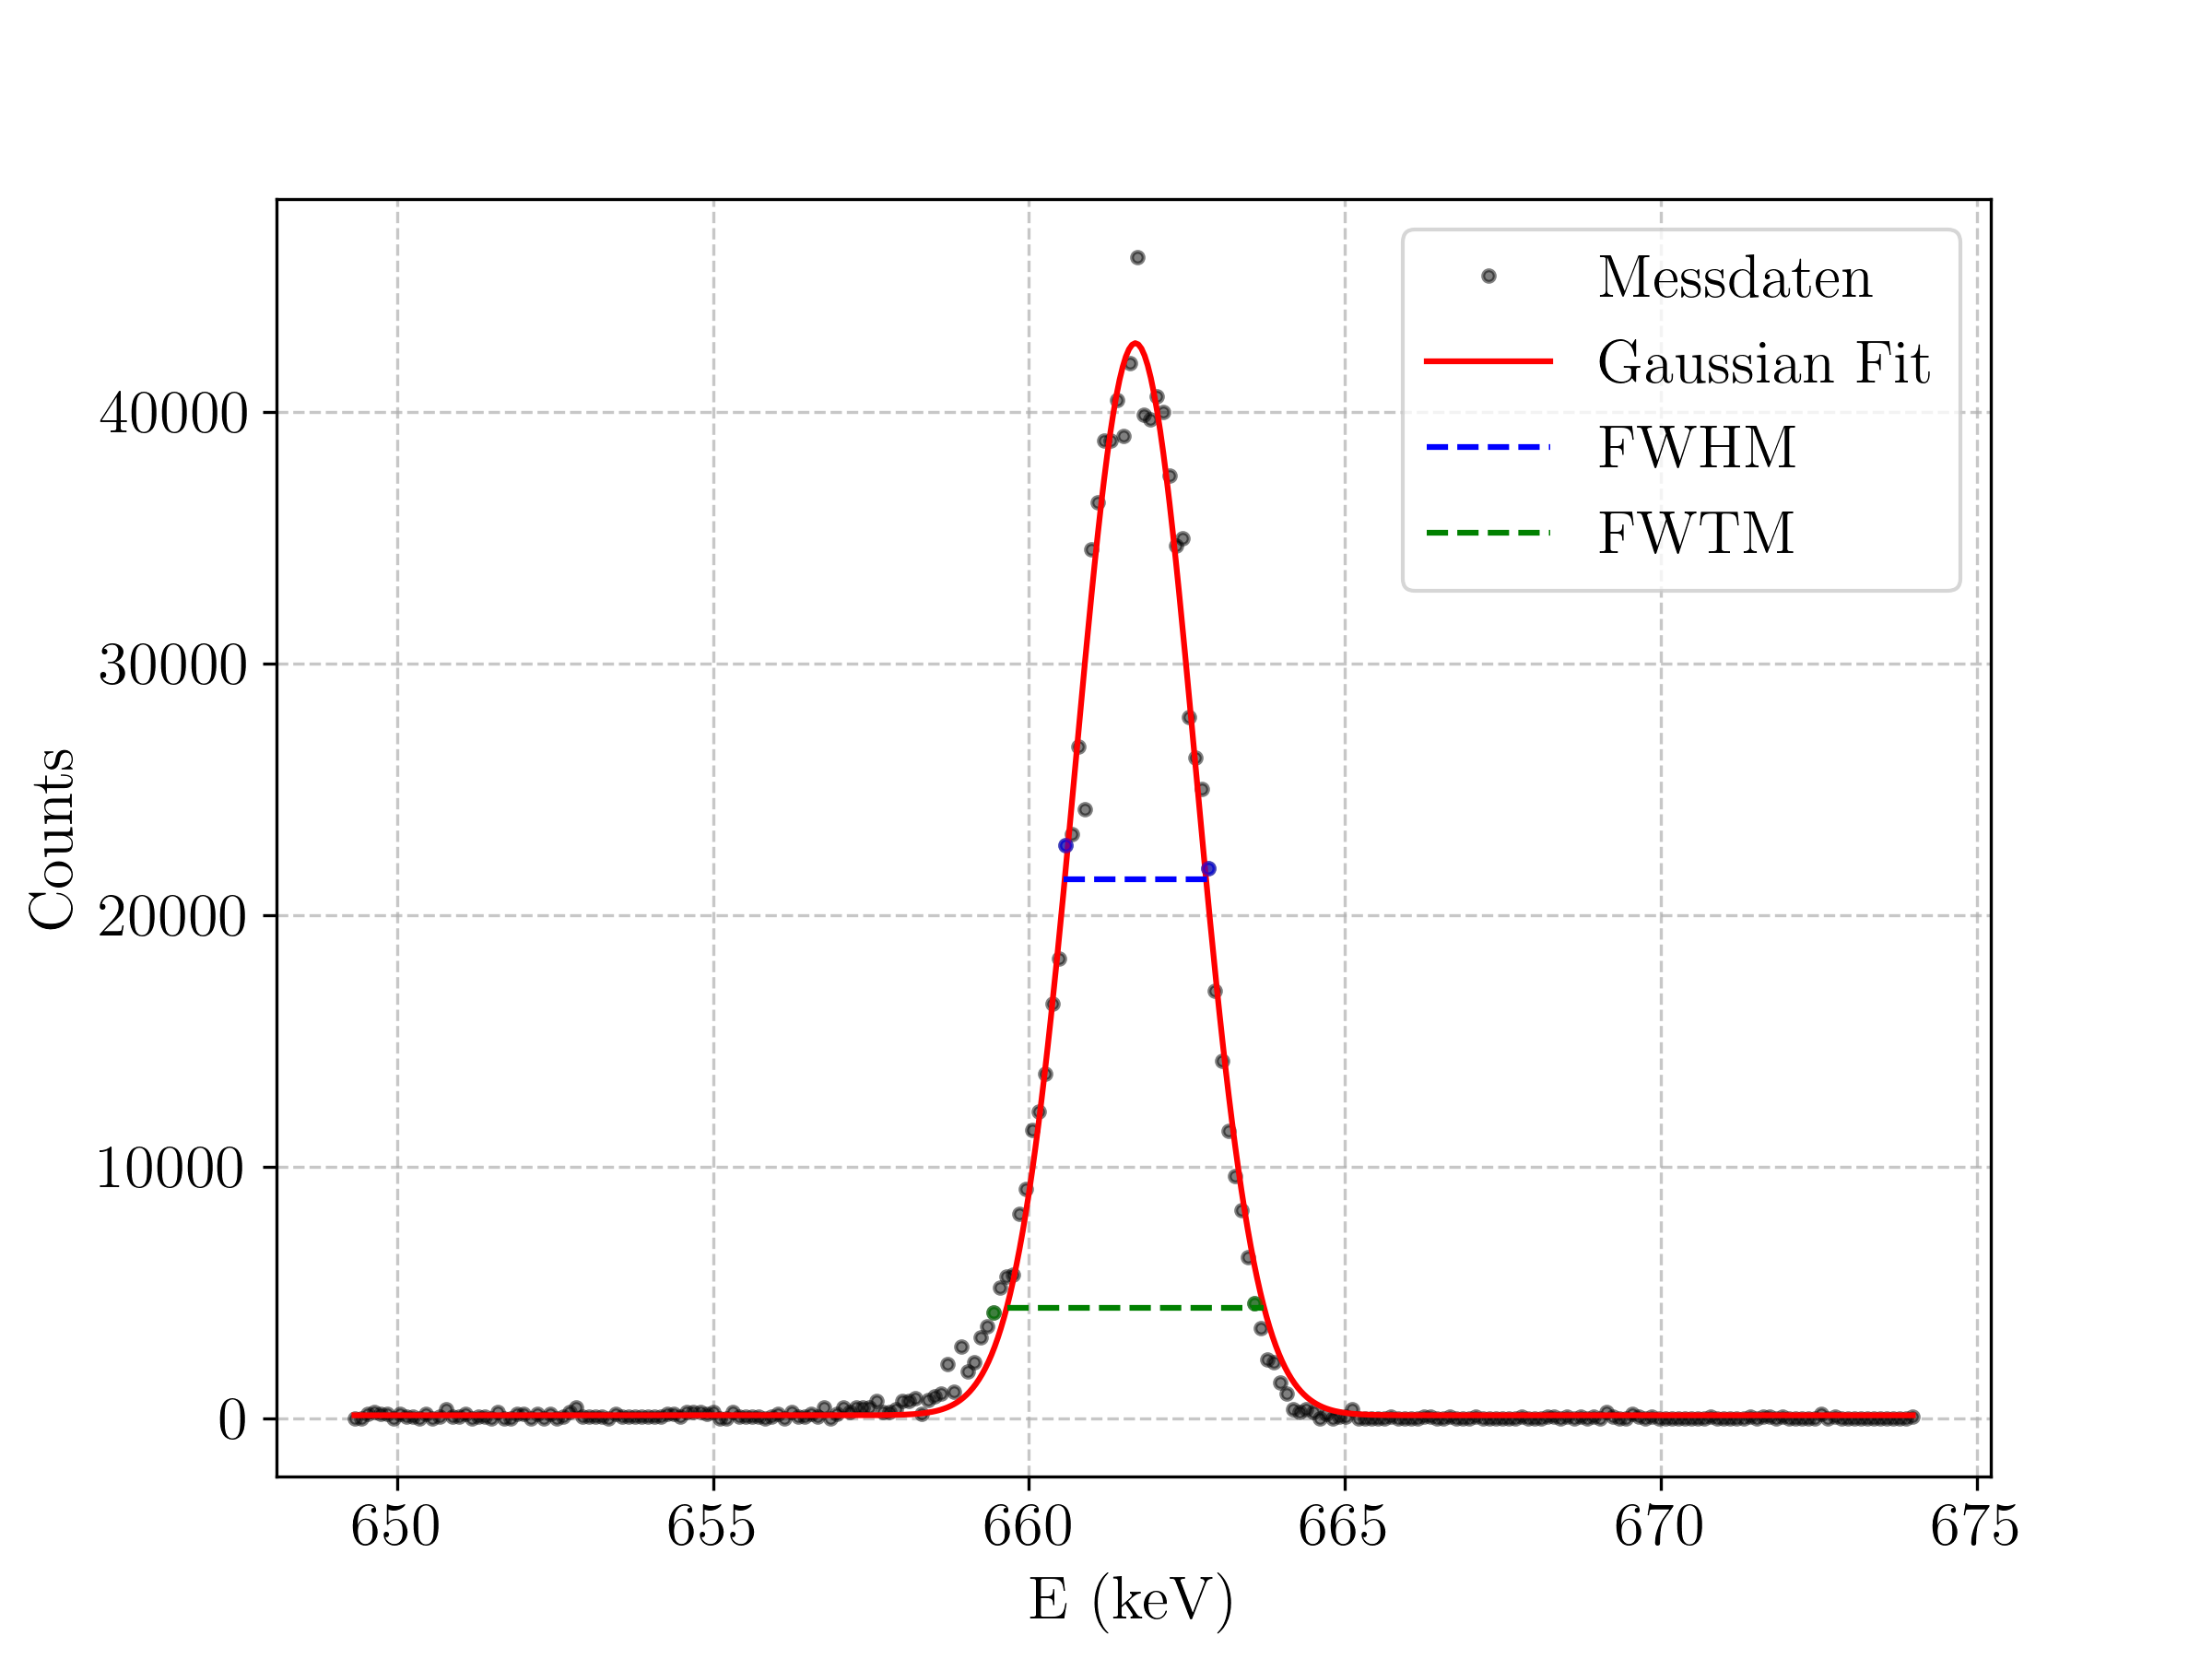
\includegraphics[scale=0.65]{Skripte/137Caesium_with_Gaussian.png}
  \caption{Full-Energy-Peak des $\text{Cs}^{137}$-Spektrums inklusive Gaussfunktion und Halb- und Zehntelwertsbreite}
  \label{fig:Cs2}
\end{figure}
Für die Gaussfunktion
\begin{align*}
  C_\text{Fit}(E)=\frac{N}{\sqrt{2\pi\sigma^2}}\cdot\exp{\left(\left(\frac{E-\mu}{\sqrt{2}\sigma}\right)^2\right)}+b
\end{align*}
ergeben sich mittels SciPy die Parameter
\begin{align*}
  N &= 101488\pm642\\
  \mu &= \SI{661.687(0.006)}{\kilo\eV}\\
  \sigma &= 0.950\pm0.006\\
  b &= 125.738\pm57.439
\end{align*}
Nun lassen sich die tatsächliche Halbwertsbreite und Zehntelwertsbreite des Detektors anhand der naheliegendsten Messpunkte bestimmen und es ergeben sich
\begin{align*}
  FWHM&=\SI{2.27}{\kilo\eV}\\
  FWTM&=\SI{4.13}{\kilo\eV}\text{,}
\end{align*}
womit das Verhältnis der beiden im Vergleich zum theoretischen Wert $\sqrt{\frac{10}{2}}\approx1.823$, welcher direkt aus der Gaussfunktion berechnet werden kann,
\begin{align*}
  \frac{FWHM}{FWTM}\approx1.818
\end{align*}
beträgt.
Anschließend kann mithilfe von \autoref{eqn:Wirkungsquerschnitt} ein Fit an den relevanten Teil der Messdaten erstellt werden, um das Compton-Kontinuum der Quelle anzunähern.
Dies ist in \autoref{fig:Cs3} dargestellt, wobei mittels \autoref{eqn:Emax} und \autoref{eqn:Eback} die Compton-Kante $\SI{477.36}{\kilo\eV}$ und der Rückstreupeak $\SI{184.33}{\kilo\eV}$ berechnet wurden.
\begin{figure}[H]
  \centering
  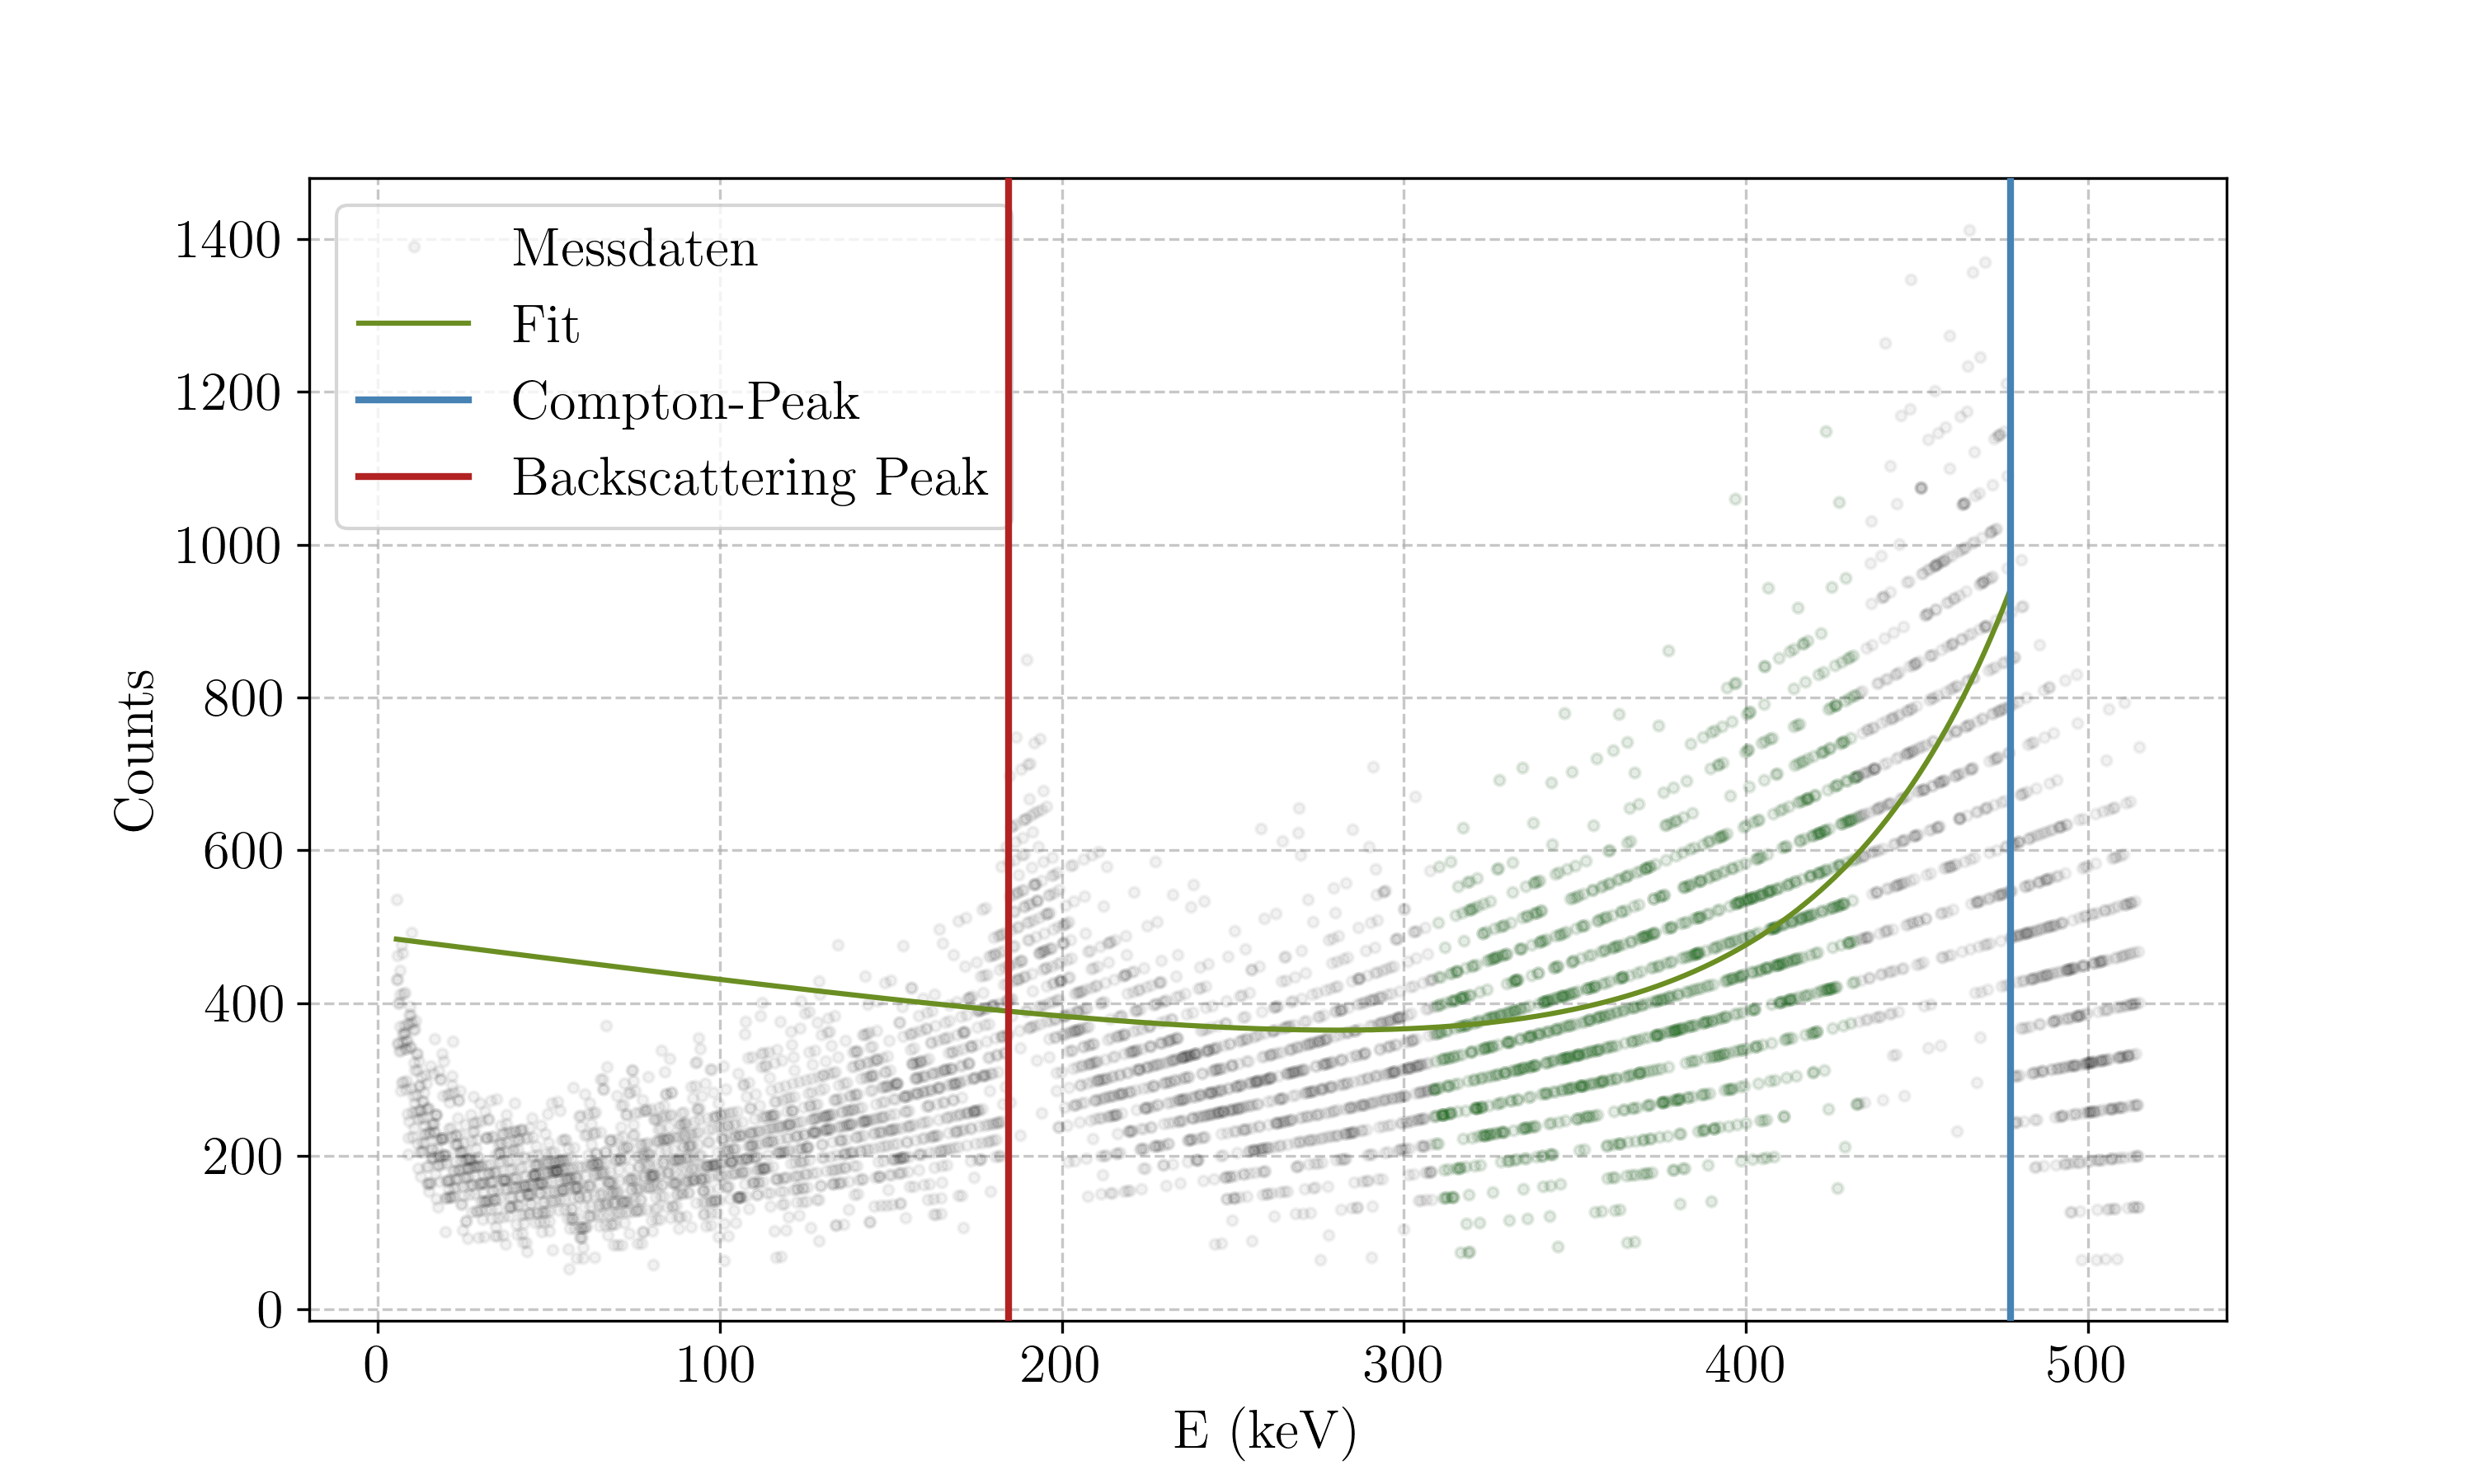
\includegraphics[scale=0.65]{Skripte/137Caesium_compton.png}
  \caption{Compton-Kontinuum der $\text{Cs}^{137}$-Quelle und zugehöriger Fit}
  \label{fig:Cs3}
\end{figure}
Die für den Fit verwendeten Messdaten sind im Plot grün hervorgehoben und es ergibt sich der Skalierungsfaktor $a=243.44\pm2.26$ und somit der Gesamtinhalt des Compton-Kontinuums $N=211607 \pm 1967$, um den Faktor $2.209\pm0.022$ größer als der Inhalt des Full-Energy-Peak.
Als Theoriewert kann mittels der aus \autoref{fig:extinkt} abgelesenen Extinktionskoeffizienten $\mu_\text{Compton}\approx\SI{0.4}{\per\centi\meter}$ und $\mu_\text{Photo}\approx\SI{0.01}{\per\centi\meter}$, eingesetzt in die Formel
\begin{align*}
  P=1-\exp(-\mu\cdot d)
\end{align*}
das Verhältnis der Absorptionswahrscheinlichkeiten zu $20.65$ bestimmt werden.
\subsection{Identifikation einer unbekannten Gamma-Quelle}
Zunächst werden wie zuvor die Peaks der Messdaten bestimmt, anschließend wird mithilfe einer in der Probe deutlich sichtbaren hell-gelben Spur die Quelle als Uran identifiziert und die Tochternuklide der Uran-Radium-Reihe betrachtet und deren Emissionsenergien sowie Intensitäten vergleichsweise in \autoref{fig:U} dargestellt\cite{IAEA_Gamma_Energies}.
\begin{figure}[H]
  \centering
  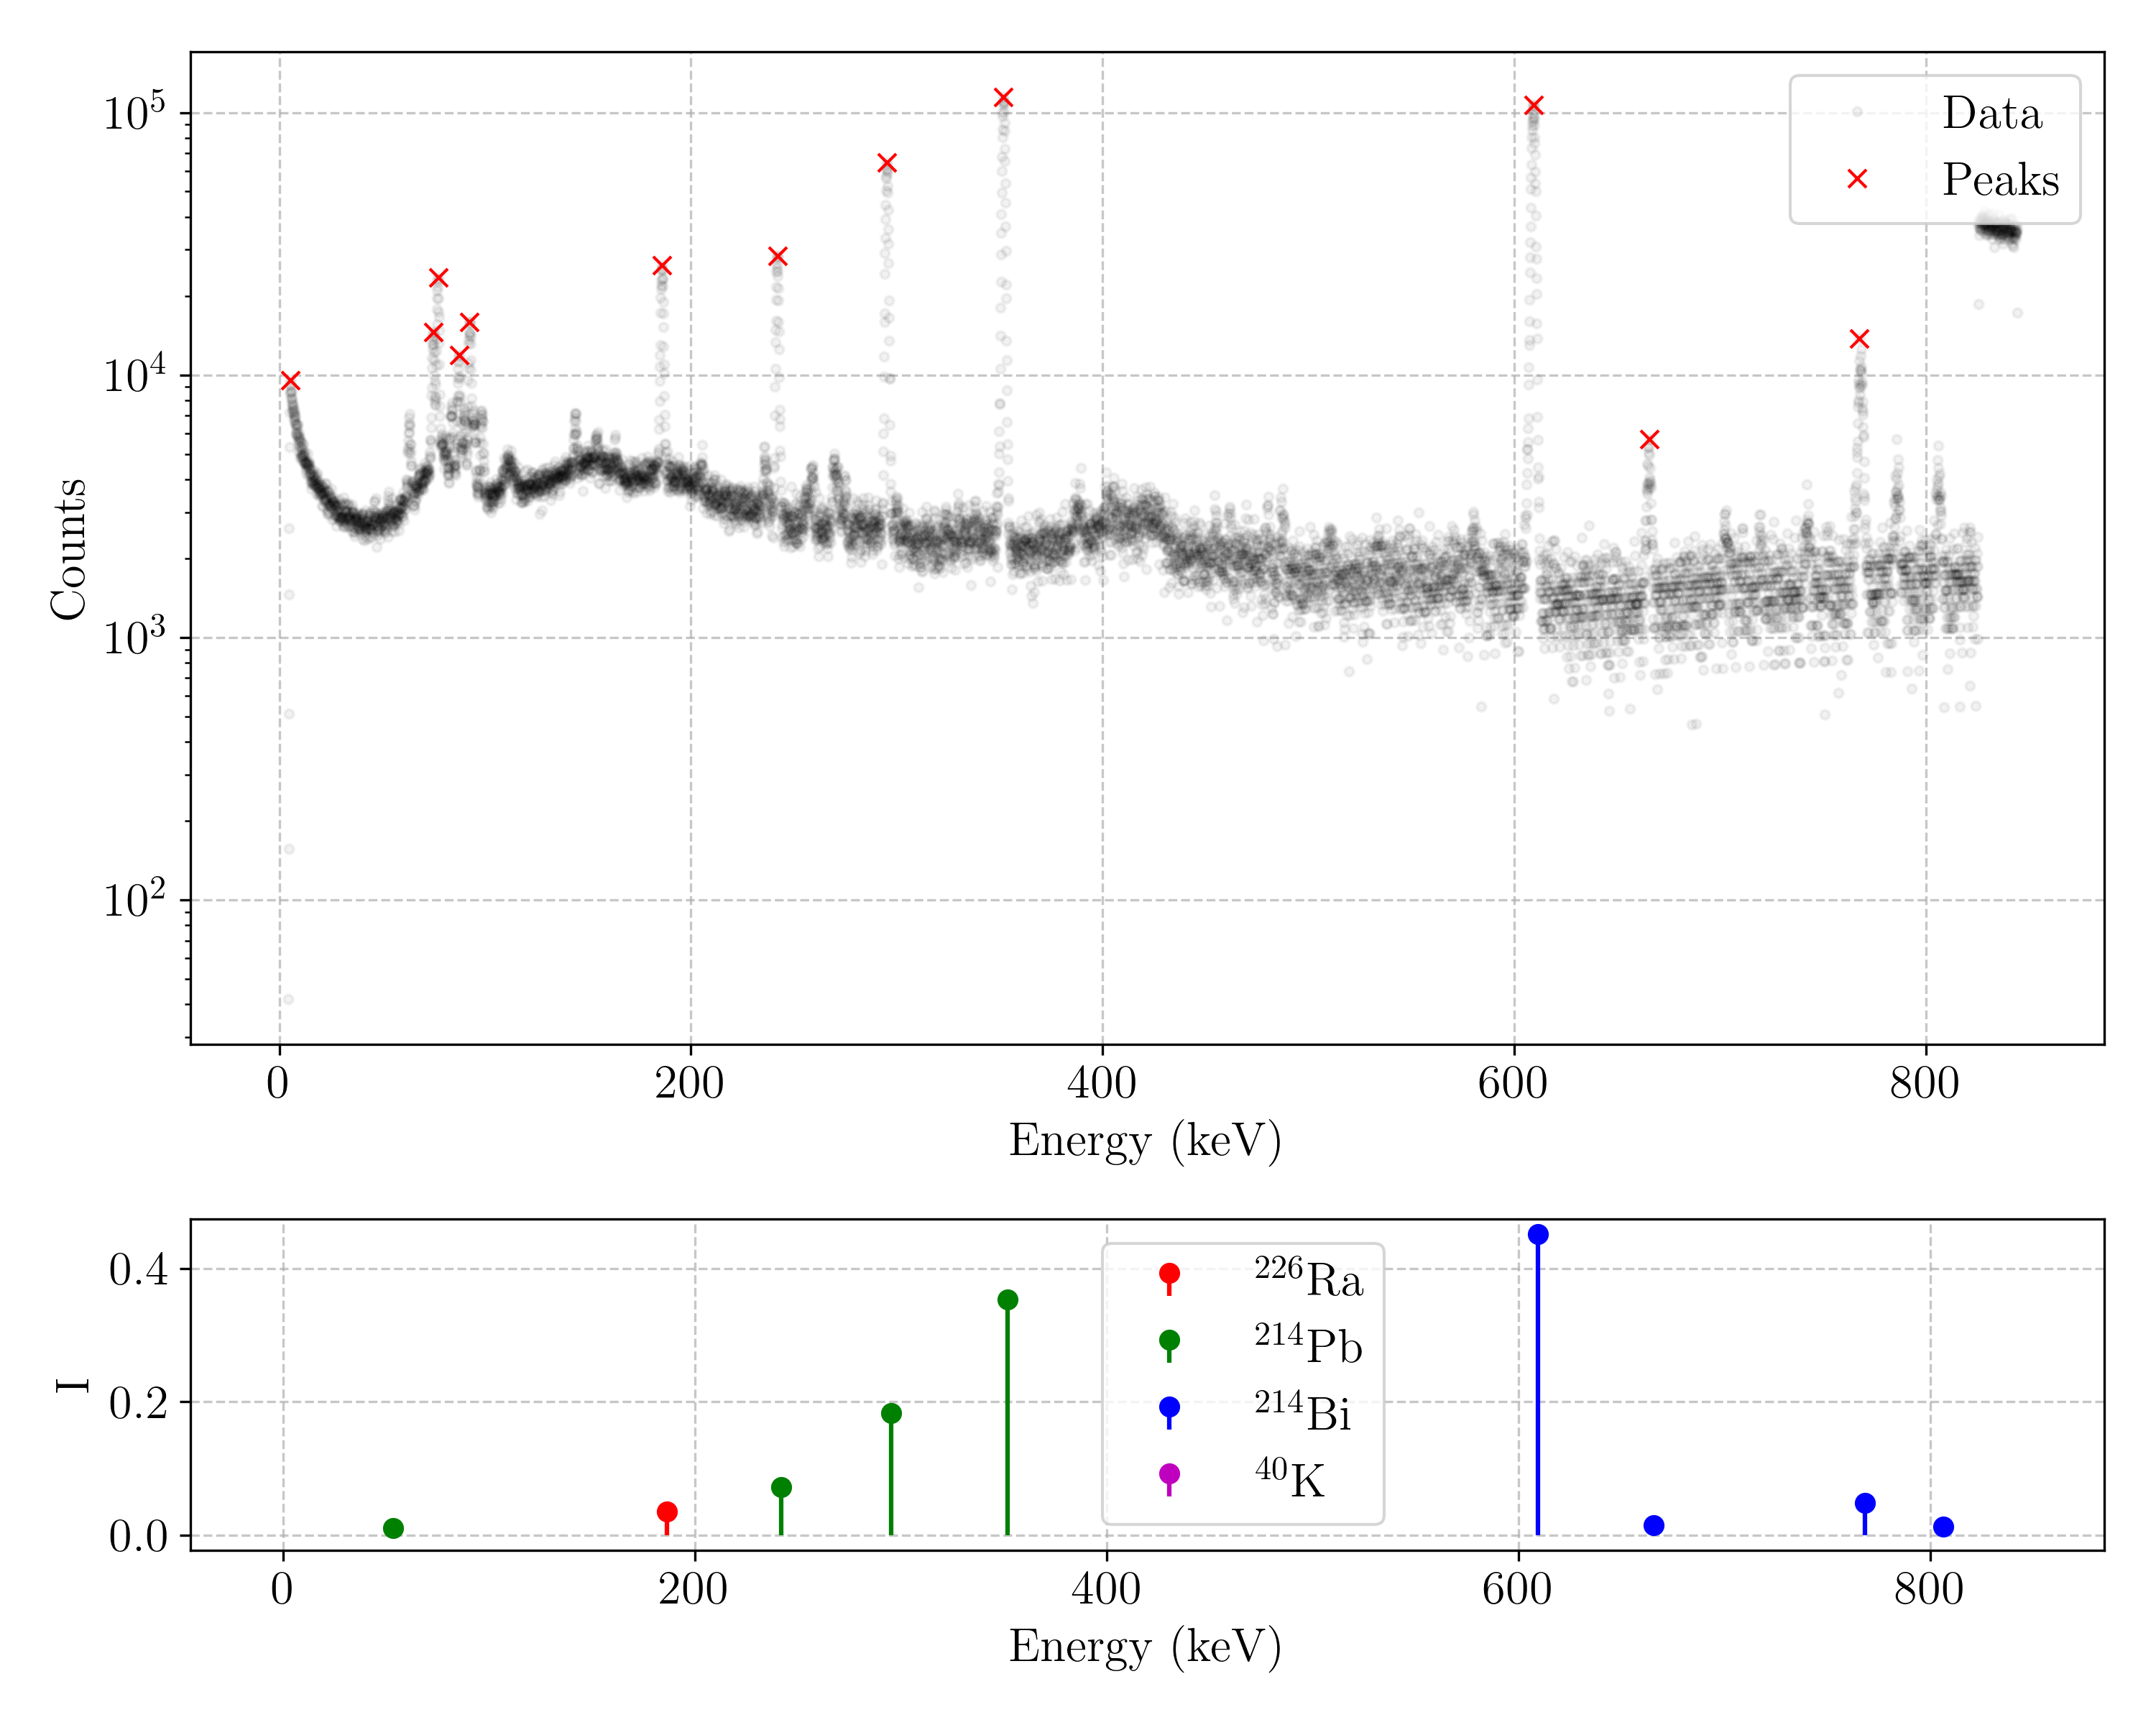
\includegraphics[scale=0.65]{Skripte/Uran_with_emission_energies.png}
  \caption{Messdaten der unbekannten Quelle und beispielhafte Emissionsenergien von $^{226}\text{Ra}$, $^{214}\text{Pb}$ und $^{214}\text{Bi}$}
  \label{fig:U}
\end{figure}
Und tatsächlich finden sich vollständige Übereinstimmungen zwischen Messdaten und Literaturwerten, womit die Vermutung als hochwahrscheinlich korrekt betrachtet werden kann, es handelt sich bei der zu untersuchenden Probe um Uranerz.
In den betrachteten Zerfallsreihen entstehen noch deutlich mehr Isotope, welche jedoch aufgrund verschiedener Gründe wie etwa zu niedrigen Emissionswahrscheinlichkeiten oder zu kurzen Halbwertszeiten nicht detektiert werden konnten.